\documentclass[a4paper, 11]{article}\usepackage[]{graphicx}\usepackage[]{color}
%% maxwidth is the original width if it is less than linewidth
%% otherwise use linewidth (to make sure the graphics do not exceed the margin)
\makeatletter
\def\maxwidth{ %
  \ifdim\Gin@nat@width>\linewidth
    \linewidth
  \else
    \Gin@nat@width
  \fi
}
\makeatother

\definecolor{fgcolor}{rgb}{0.345, 0.345, 0.345}
\newcommand{\hlnum}[1]{\textcolor[rgb]{0.686,0.059,0.569}{#1}}%
\newcommand{\hlstr}[1]{\textcolor[rgb]{0.192,0.494,0.8}{#1}}%
\newcommand{\hlcom}[1]{\textcolor[rgb]{0.678,0.584,0.686}{\textit{#1}}}%
\newcommand{\hlopt}[1]{\textcolor[rgb]{0,0,0}{#1}}%
\newcommand{\hlstd}[1]{\textcolor[rgb]{0.345,0.345,0.345}{#1}}%
\newcommand{\hlkwa}[1]{\textcolor[rgb]{0.161,0.373,0.58}{\textbf{#1}}}%
\newcommand{\hlkwb}[1]{\textcolor[rgb]{0.69,0.353,0.396}{#1}}%
\newcommand{\hlkwc}[1]{\textcolor[rgb]{0.333,0.667,0.333}{#1}}%
\newcommand{\hlkwd}[1]{\textcolor[rgb]{0.737,0.353,0.396}{\textbf{#1}}}%

\usepackage{framed}
\makeatletter
\newenvironment{kframe}{%
 \def\at@end@of@kframe{}%
 \ifinner\ifhmode%
  \def\at@end@of@kframe{\end{minipage}}%
  \begin{minipage}{\columnwidth}%
 \fi\fi%
 \def\FrameCommand##1{\hskip\@totalleftmargin \hskip-\fboxsep
 \colorbox{shadecolor}{##1}\hskip-\fboxsep
     % There is no \\@totalrightmargin, so:
     \hskip-\linewidth \hskip-\@totalleftmargin \hskip\columnwidth}%
 \MakeFramed {\advance\hsize-\width
   \@totalleftmargin\z@ \linewidth\hsize
   \@setminipage}}%
 {\par\unskip\endMakeFramed%
 \at@end@of@kframe}
\makeatother

\definecolor{shadecolor}{rgb}{.97, .97, .97}
\definecolor{messagecolor}{rgb}{0, 0, 0}
\definecolor{warningcolor}{rgb}{1, 0, 1}
\definecolor{errorcolor}{rgb}{1, 0, 0}
\newenvironment{knitrout}{}{} % an empty environment to be redefined in TeX

\usepackage{alltt}
\usepackage[utf8]{inputenc}
\usepackage{fullpage}
\usepackage{pdflscape}
\usepackage{graphicx}
\usepackage{float}
\usepackage{rotating}
\usepackage{longtable}
%\usepackage{showframe}
\graphicspath{ {images/} }
\IfFileExists{upquote.sty}{\usepackage{upquote}}{}
\begin{document}
	\title{
	{Supplementary material for the manuscript}\\
	{\large Analysis of lichenicolous fungal communities based on ITS1 Amplicon Sequencing data}\\
	}
\author{Antonia Fleischhacker, Fernando Fernandez-Mendoza, Lucia Muggia}
\date{\today}
\maketitle
\tableofcontents{}
\section{Introduction}

 After all reads were quality filtered and clusterd using a 97\% similarity treshold to incorporate more sequencing error than it is included in simple dereplication approaches,
 all Analyses were run using two separate workflows. First we used a straightforward approach in which sequences were BLASTED against nr database
 and subsequently analysed in MEGAN to obtain a wide taxonomic profile based on LCA estimates. Secondly we used a more thorough approach in which we filtered out 
 and extracted the ITS1 fragment using the program ITSx, clustered the ITS1 fragments using SWARM, blasted them to the UNITE database of fungal ribosomal DNA
 and finally summarized the BLAST output using a custom script in R.\\
\newpage
%
% FIRST CHUNK PREPARES THE R ENVIRONMENT AND LOADS DATA AND FUNCTIONS
%
\section{Quality assesment and depth of the dataset used}
%
% SECOND CHUNK GETS AN OVERVIEW OF THE UNTRIMMED DATASET
%

%
% 3rd CHUNK GETS AN OVERVIEW OF THE ITS1 DATASET AND PLOTS BOTH DATASETS IN ONE PLOT
%
\begin{knitrout}
\definecolor{shadecolor}{rgb}{0.969, 0.969, 0.969}\color{fgcolor}\begin{figure}[H]
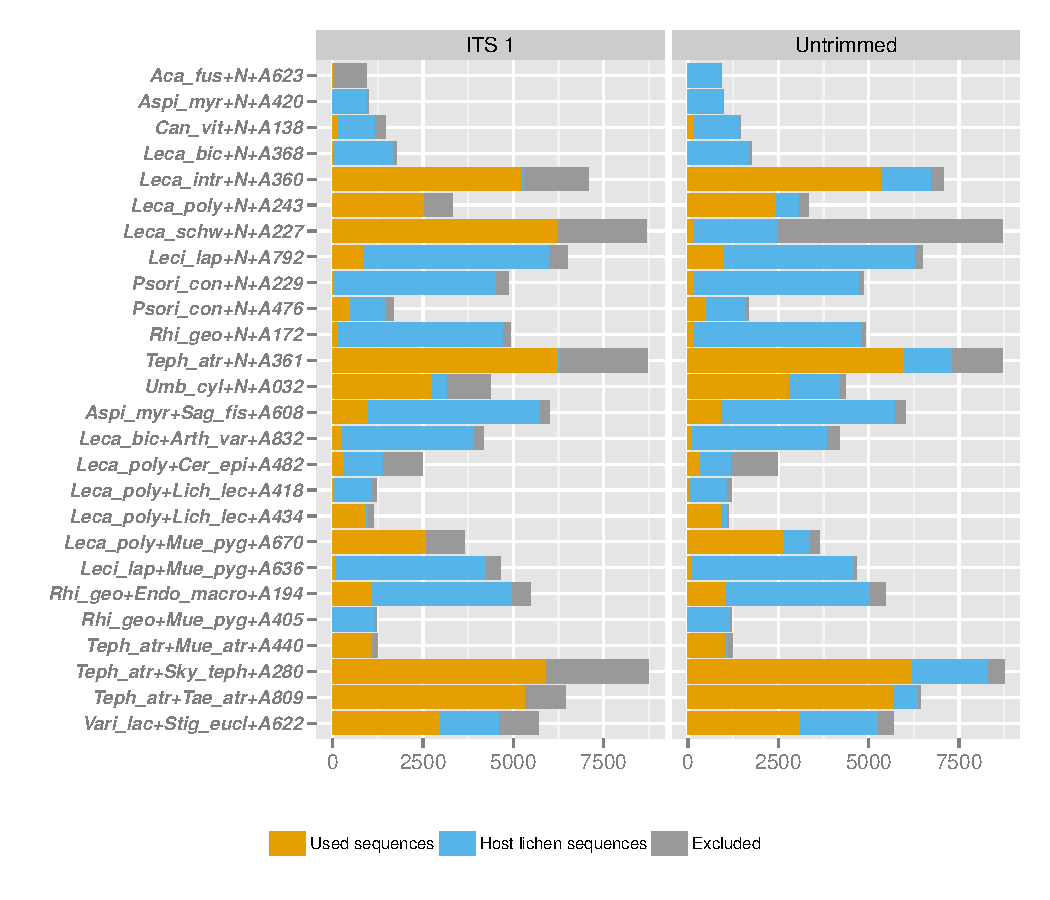
\includegraphics[width=\maxwidth]{figure/3_Introitsx-1} \caption[Overview of the trimmed (ITS1) and untrimmed datasets]{Overview of the trimmed (ITS1) and untrimmed datasets. The bars show the numer of reads per sample, and color codes the sequences that were included and excluded in each analysis}\label{fig:3_Introitsx}
\end{figure}


\end{knitrout}
\begin{knitrout}
\definecolor{shadecolor}{rgb}{0.969, 0.969, 0.969}\color{fgcolor}\begin{figure}[H]
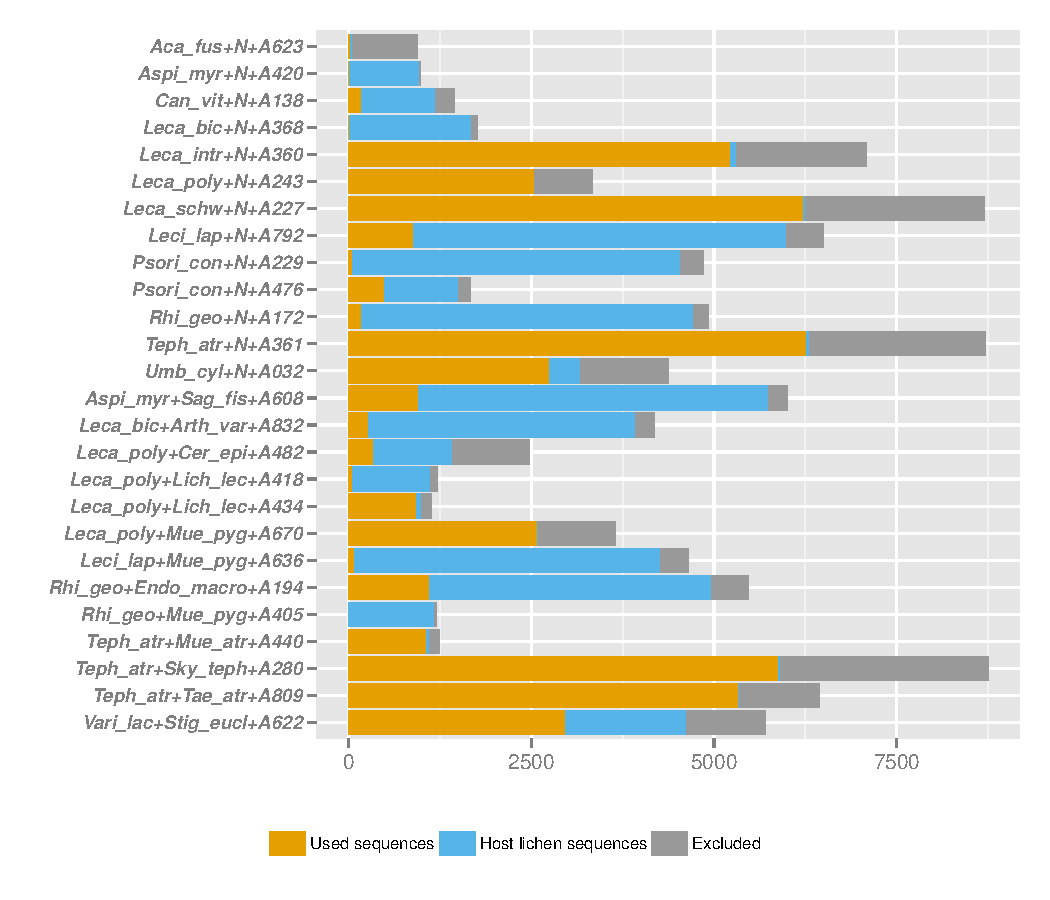
\includegraphics[width=\maxwidth]{figure/3A_Fig1-1} \caption[Overview of the trimmed ITS1 dataset]{Overview of the trimmed ITS1 dataset. The bars show the numer of reads per sample, and color codes the sequences that were included and excluded in each analysis}\label{fig:3A_Fig1}
\end{figure}


\end{knitrout}
%
%
%
%
%
%
%
%
%
% TEXT ON QUALITY OF THE DATASET
%
Analyses carried out in MEGAN including all quality filtered and dereplicated amplicons.\\
Each sequence may include more an incomplete 5' fraction of SSU, including type I intronic sequences when present, ITS1 and 5.8S. When the type I intron is present the sequence of ITS1 is eaither partial or non existent.
Unknown and Bacterial sequences are further interpreted as "unknown/unused".

Representation of the dataset after being processes using ITSx. Sequences excluded because the do not contain ITS1 fractions are
gruped as 11. 01 refers to sequences excluded for the analyses which contain ITS1 but are positively identified as belonging to one of the studied lichen hosts. 00 is the fraction of sequences included.\\


\newpage
\section{Taxonomic profile of the samples}
\subsection{Division}
%
% PLOT DIVISION COMPOSITION
%
\begin{knitrout}
\definecolor{shadecolor}{rgb}{0.969, 0.969, 0.969}\color{fgcolor}\begin{figure}[H]
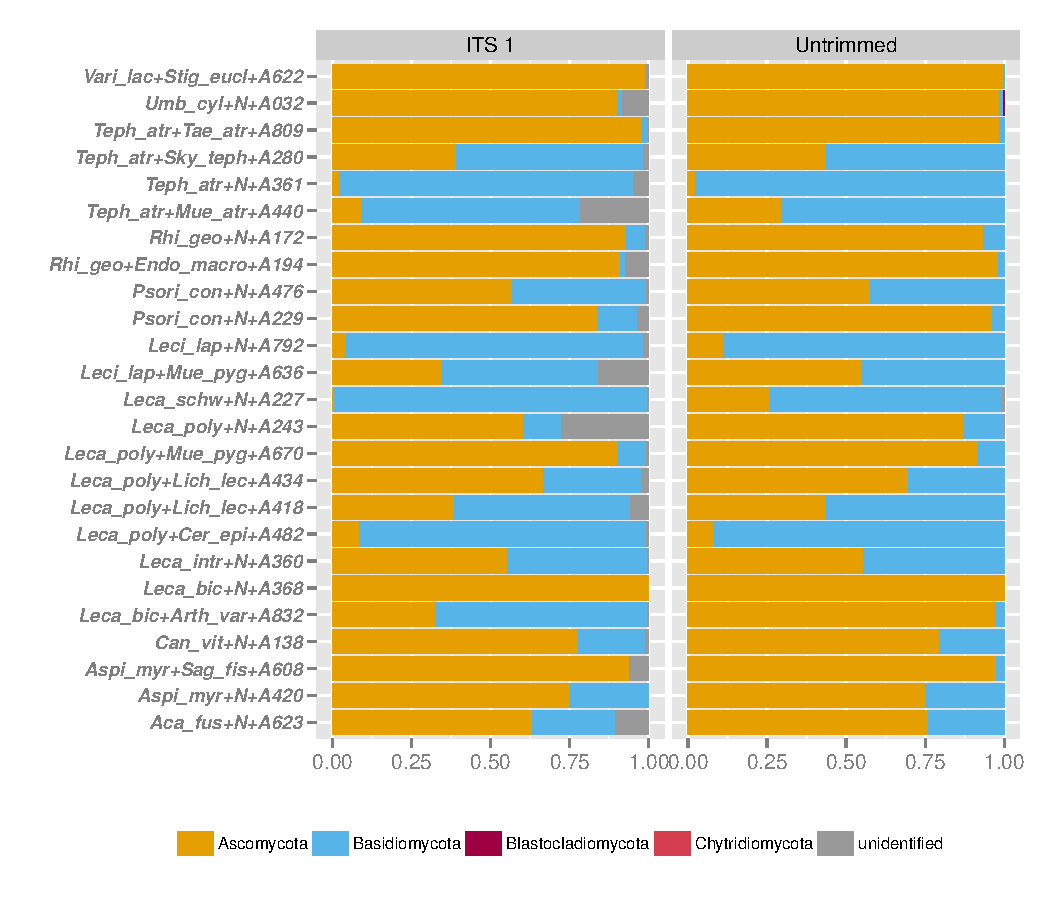
\includegraphics[width=\maxwidth]{figure/4_divisions-1} \caption[Overview of Taxonomic composition at Division level of the untrimmed dataset (SSU, Type I intron, ITS1, 5]{Overview of Taxonomic composition at Division level of the untrimmed dataset (SSU, Type I intron, ITS1, 5.8S) and the ITS1 dataset.}\label{fig:4_divisions}
\end{figure}


\end{knitrout}
%
%
% PLOT TABLES OF DIVISION COMPOSITION
%
%
% latex table generated in R 3.0.3 by xtable 1.7-4 package
% Tue Feb  7 12:19:58 2017
\begin{table}[H]
\centering
\caption[Divisions ITS1]{Number of raw reads asignable to Fungal Divisions in the ITS1 dataset} 
\begin{tabular}{rrrrr}
  \hline
 & Ascomycota & Basidiomycota & Chytridiomycota & unidentified \\ 
  \hline
Aca\_fus+N+A623 & 12 & 5 & . & 2 \\ 
  Aspi\_myr+N+A420 & 3 & 1 & . & . \\ 
  Aspi\_myr+Sag\_fis+A608 & 900 & . & . & 58 \\ 
  Can\_vit+N+A138 & 135 & 37 & . & 2 \\ 
  Leca\_bic+Arth\_var+A832 & 89 & 183 & . & 1 \\ 
  Leca\_bic+N+A368 & 16 & . & . & . \\ 
  Leca\_intr+N+A360 & 2885 & 2310 & . & 27 \\ 
  Leca\_poly+Cer\_epi+A482 & 29 & 311 & . & 3 \\ 
  Leca\_poly+Lich\_lec+A418 & 20 & 29 & . & 3 \\ 
  Leca\_poly+Lich\_lec+A434 & 620 & 289 & . & 20 \\ 
  Leca\_poly+Mue\_pyg+A670 & 2330 & 237 & . & 21 \\ 
  Leca\_poly+N+A243 & 1533 & 305 & . & 702 \\ 
  Leca\_schw+N+A227 & 41 & 6164 & . & 21 \\ 
  Leci\_lap+Mue\_pyg+A636 & 28 & 40 & . & 13 \\ 
  Leci\_lap+N+A792 & 40 & 836 & . & 16 \\ 
  Psori\_con+N+A229 & 46 & 7 & . & 2 \\ 
  Psori\_con+N+A476 & 275 & 205 & . & 3 \\ 
  Rhi\_geo+Endo\_macro+A194 & 1008 & 19 & . & 80 \\ 
  Rhi\_geo+N+A172 & 162 & 11 & . & 2 \\ 
  Teph\_atr+Mue\_atr+A440 & 98 & 741 & . & 231 \\ 
  Teph\_atr+N+A361 & 134 & 5822 & . & 305 \\ 
  Teph\_atr+Sky\_teph+A280 & 2302 & 3486 & . & 100 \\ 
  Teph\_atr+Tae\_atr+A809 & 5229 & 88 & . & 13 \\ 
  Umb\_cyl+N+A032 & 2470 & 45 & 1 & 228 \\ 
  Vari\_lac+Stig\_eucl+A622 & 2933 & 11 & . & 24 \\ 
   \hline
\end{tabular}
\end{table}

% latex table generated in R 3.0.3 by xtable 1.7-4 package
% Tue Feb  7 12:19:58 2017
\begin{table}[H]
\centering
\caption[Divisions MEGAN]{Number of reads asignable to Fungal Divisions in the untrimmed dataset} 
\begin{tabular}{rrrrr}
  \hline
 & Ascomycota & Basidiomycota & Blastocladiomycota & Unknown \\ 
  \hline
Aca\_fus+N+A623 & 16 & 5 & . & . \\ 
  Aspi\_myr+N+A420 & 3 & 1 & . & . \\ 
  Aspi\_myr+Sag\_fis+A608 & 912 & 22 & . & . \\ 
  Can\_vit+N+A138 & 149 & 38 & . & . \\ 
  Leca\_bic+Arth\_var+A832 & 103 & 3 & . & . \\ 
  Leca\_bic+N+A368 & 16 & . & . & . \\ 
  Leca\_intr+N+A360 & 2969 & 2374 & . & . \\ 
  Leca\_poly+Cer\_epi+A482 & 30 & 321 & . & . \\ 
  Leca\_poly+Lich\_lec+A418 & 23 & 30 & . & . \\ 
  Leca\_poly+Lich\_lec+A434 & 672 & 291 & . & . \\ 
  Leca\_poly+Mue\_pyg+A670 & 2417 & 224 & . & . \\ 
  Leca\_poly+N+A243 & 2138 & 314 & . & 1 \\ 
  Leca\_schw+N+A227 & 46 & 130 & . & 1 \\ 
  Leci\_lap+Mue\_pyg+A636 & 55 & 45 & . & . \\ 
  Leci\_lap+N+A792 & 109 & 873 & . & . \\ 
  Psori\_con+N+A229 & 184 & 7 & . & . \\ 
  Psori\_con+N+A476 & 290 & 212 & . & . \\ 
  Rhi\_geo+Endo\_macro+A194 & 1036 & 19 & . & . \\ 
  Rhi\_geo+N+A172 & 170 & 12 & . & . \\ 
  Teph\_atr+Mue\_atr+A440 & 310 & 741 & . & . \\ 
  Teph\_atr+N+A361 & 142 & 5821 & . & . \\ 
  Teph\_atr+Sky\_teph+A280 & 2708 & 3491 & . & . \\ 
  Teph\_atr+Tae\_atr+A809 & 5611 & 89 & . & . \\ 
  Umb\_cyl+N+A032 & 2775 & 40 & 2 & . \\ 
  Vari\_lac+Stig\_eucl+A622 & 3070 & 11 & . & . \\ 
   \hline
\end{tabular}
\end{table}

\newpage
\subsection{Classes}
%
% PLOT IMAGES AND TABLES OF CLASS COMPOSITION
%
\begin{knitrout}
\definecolor{shadecolor}{rgb}{0.969, 0.969, 0.969}\color{fgcolor}\begin{figure}[H]
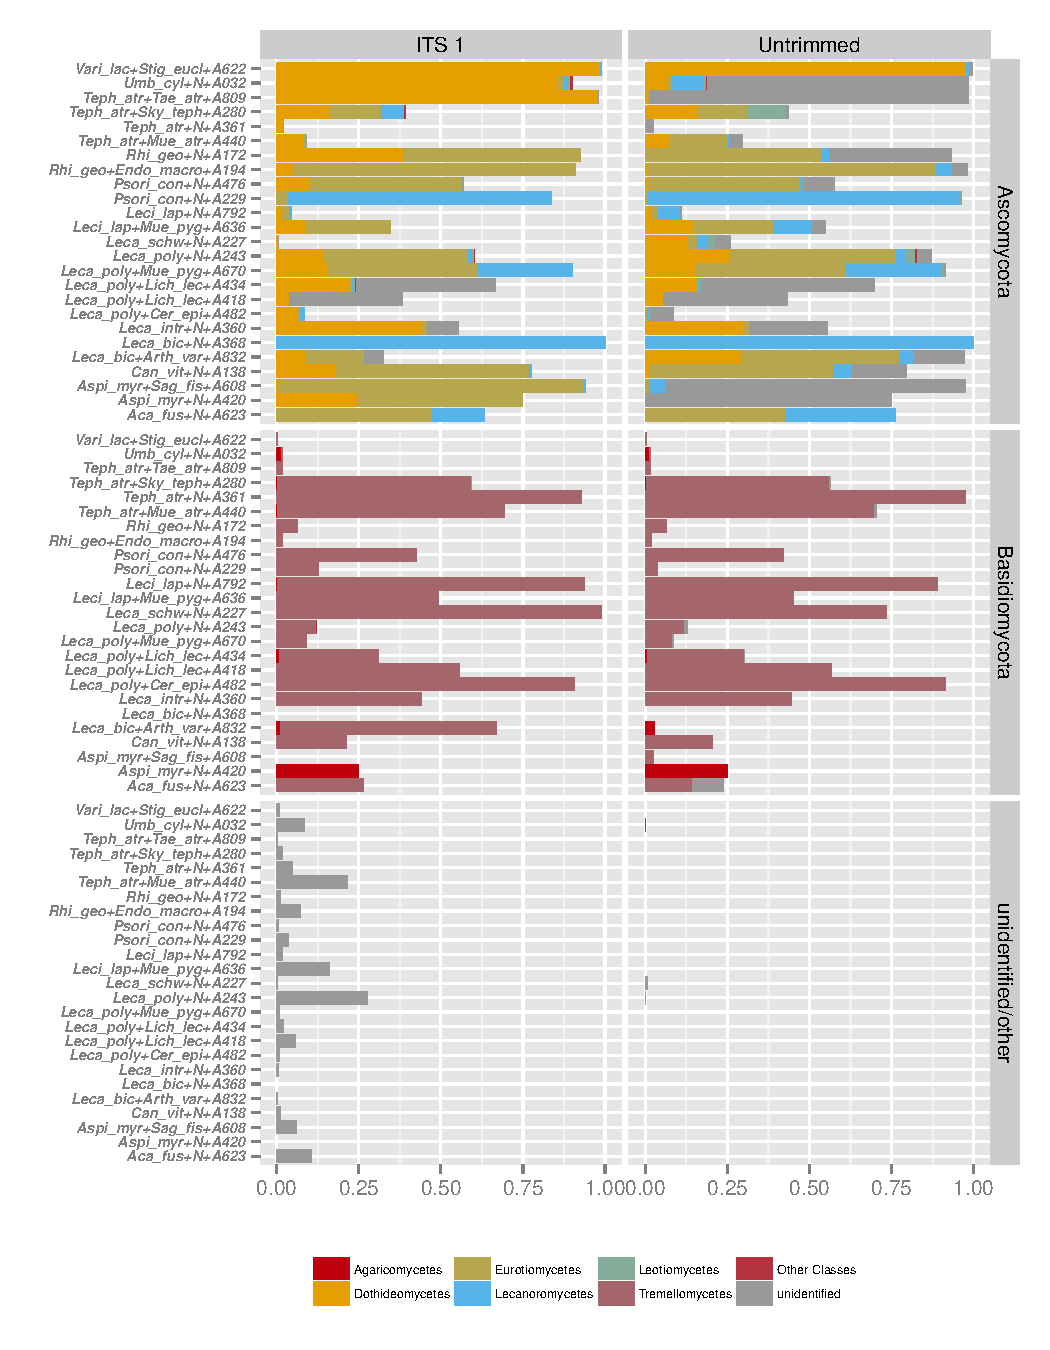
\includegraphics[width=\maxwidth]{figure/7_Class-1} \caption[Taxonomic composition at Class level of the untrimmed (SSU, Type I intron, ITS1, 5]{Taxonomic composition at Class level of the untrimmed (SSU, Type I intron, ITS1, 5.8S) and ITS1 datasets. Normalized fractions per sample are split by dataset and Division. The minoritary Blastocladiomycota and Chytridiomycota are grouped in the "unidentified/others" category }\label{fig:7_Class}
\end{figure}


\end{knitrout}
%
% CLASS TABLES
%
% latex table generated in R 3.0.3 by xtable 1.7-4 package
% Tue Feb  7 12:19:59 2017
\begin{sidewaystable}[b]
\centering
\caption[Classes ITS1]{Proportion of sequences asignable to Fungal Classes in the trimmed ITS1 dataset} 
\begin{tabular}{rrrrrrrrrrrrr}
  \hline
 & \begin{sideways} Dothideomycetes \end{sideways} & \begin{sideways} Eurotiomycetes \end{sideways} & \begin{sideways} Lecanoromycetes \end{sideways} & \begin{sideways} Leotiomycetes \end{sideways} & \begin{sideways} Saccharomycetes \end{sideways} & \begin{sideways} Sordariomycetes \end{sideways} & \begin{sideways} Taphrinomycetes \end{sideways} & \begin{sideways} Agaricomycetes \end{sideways} & \begin{sideways} Microbotryomycetes \end{sideways} & \begin{sideways} Tremellomycetes \end{sideways} & \begin{sideways} Blastocladiomycetes \end{sideways} & \begin{sideways} unidentified \end{sideways} \\ 
  \hline
Aca\_fus+N+A623 & . & 9 & 3 & . & . & . & . & . & . & 5 & . & 2 \\ 
  Aspi\_myr+N+A420 & 1 & 2 & . & . & . & . & . & 1 & . & . & . & . \\ 
  Aspi\_myr+Sag\_fis+A608 & 2 & 896 & 2 & . & . & . & . & . & . & . & . & 58 \\ 
  Can\_vit+N+A138 & 31 & 103 & 1 & . & . & . & . & . & . & 37 & . & 2 \\ 
  Leca\_bic+Arth\_var+A832 & 25 & 48 & . & . & . & . & . & 3 & . & 180 & . & 17 \\ 
  Leca\_bic+N+A368 & . & . & 16 & . & . & . & . & . & . & . & . & . \\ 
  Leca\_intr+N+A360 & 2326 & 77 & 1 & . & . & . & . & 1 & . & 2309 & . & 508 \\ 
  Leca\_poly+Cer\_epi+A482 & 23 & 1 & 5 & . & . & . & . & . & . & 311 & . & 3 \\ 
  Leca\_poly+Lich\_lec+A418 & 2 & . & . & . & . & . & . & . & . & 29 & . & 21 \\ 
  Leca\_poly+Lich\_lec+A434 & 210 & 4 & 7 & 2 & . & 3 & . & 7 & . & 282 & . & 414 \\ 
  Leca\_poly+Mue\_pyg+A670 & 405 & 1177 & 748 & . & . & . & . & . & . & 237 & . & 21 \\ 
  Leca\_poly+N+A243 & 358 & 1125 & 32 & 16 & . & 2 & . & 1 & 1 & 303 & . & 702 \\ 
  Leca\_schw+N+A227 & 25 & 10 & 3 & 1 & . & . & . & . & . & 6164 & . & 23 \\ 
  Leci\_lap+Mue\_pyg+A636 & 7 & 21 & . & . & . & . & . & . & . & 40 & . & 13 \\ 
  Leci\_lap+N+A792 & 16 & 20 & 3 & . & . & . & . & 1 & . & 835 & . & 17 \\ 
  Psori\_con+N+A229 & . & 2 & 44 & . & . & . & . & . & . & 7 & . & 2 \\ 
  Psori\_con+N+A476 & 50 & 224 & . & . & . & . & . & . & . & 205 & . & 4 \\ 
  Rhi\_geo+Endo\_macro+A194 & 55 & 953 & . & . & . & . & . & . & . & 19 & . & 80 \\ 
  Rhi\_geo+N+A172 & 68 & 94 & . & . & . & . & . & . & . & 11 & . & 2 \\ 
  Teph\_atr+Mue\_atr+A440 & 90 & 4 & 1 & 3 & . & . & . & 1 & . & 740 & . & 231 \\ 
  Teph\_atr+N+A361 & 132 & 1 & . & . & . & . & . & . & . & 5822 & . & 306 \\ 
  Teph\_atr+Sky\_teph+A280 & 972 & 901 & 425 & . & . & . & 4 & 15 & . & 3470 & . & 101 \\ 
  Teph\_atr+Tae\_atr+A809 & 5226 & 2 & . & . & . & . & . & 1 & . & 87 & . & 14 \\ 
  Umb\_cyl+N+A032 & 2352 & 49 & 29 & 22 & 1 & 17 & . & 38 & . & 7 & 1 & 228 \\ 
  Vari\_lac+Stig\_eucl+A622 & 2921 & 6 & 6 & . & . & . & . & 1 & . & 10 & . & 24 \\ 
   \hline
\end{tabular}
\end{sidewaystable}


% latex table generated in R 3.0.3 by xtable 1.7-4 package
% Tue Feb  7 12:19:59 2017
\begin{sidewaystable}[b]
\centering
\caption[Classes MEGAN]{Proportion of sequences asignable to Fungal Classes in the Complete dataset} 
\begin{tabular}{rrrrrrrrrrrrrrr}
  \hline
 & \begin{sideways} Dothideomycetes \end{sideways} & \begin{sideways} Eurotiomycetes \end{sideways} & \begin{sideways} Lecanoromycetes \end{sideways} & \begin{sideways} Leotiomycetes \end{sideways} & \begin{sideways} Orbiliomycetes \end{sideways} & \begin{sideways} Saccharomycetes \end{sideways} & \begin{sideways} Sordariomycetes \end{sideways} & \begin{sideways} Taphrinomycetes \end{sideways} & \begin{sideways} Agaricomycetes \end{sideways} & \begin{sideways} Agaricostilbomycetes \end{sideways} & \begin{sideways} Malasseziomycetes \end{sideways} & \begin{sideways} Tremellomycetes \end{sideways} & \begin{sideways} Blastocladiomycetes \end{sideways} & \begin{sideways} Unknown \end{sideways} \\ 
  \hline
Aca\_fus+N+A623 & . & 9 & 7 & . & . & . & . & . & . & . & . & 3 & . & 2 \\ 
  Aspi\_myr+N+A420 & . & . & . & . & . & . & . & . & 1 & . & . & . & . & 3 \\ 
  Aspi\_myr+Sag\_fis+A608 & 1 & 11 & 44 & . & . & . & . & . & . & . & . & 22 & . & 856 \\ 
  Can\_vit+N+A138 & 3 & 104 & 11 & . & . & . & . & . & . & . & . & 38 & . & 31 \\ 
  Leca\_bic+Arth\_var+A832 & 31 & 51 & 5 & . & . & . & . & . & 3 & . & . & . & . & 16 \\ 
  Leca\_bic+N+A368 & . & . & 16 & . & . & . & . & . & . & . & . & . & . & . \\ 
  Leca\_intr+N+A360 & 1613 & 80 & 10 & . & . & . & . & . & 1 & . & . & 2373 & . & 1266 \\ 
  Leca\_poly+Cer\_epi+A482 & 1 & 1 & 4 & . & . & . & . & . & . & . & . & 321 & . & 24 \\ 
  Leca\_poly+Lich\_lec+A418 & 3 & . & . & . & . & . & . & . & . & . & . & 30 & . & 20 \\ 
  Leca\_poly+Lich\_lec+A434 & 154 & . & 9 & 1 & . & . & . & . & 7 & . & . & 283 & . & 509 \\ 
  Leca\_poly+Mue\_pyg+A670 & 408 & 1213 & 773 & 6 & . & . & 1 & . & . & . & . & 222 & . & 18 \\ 
  Leca\_poly+N+A243 & 633 & 1242 & 68 & 76 & 9 & . & 2 & . & 1 & 1 & . & 292 & . & 129 \\ 
  Leca\_schw+N+A227 & 23 & 5 & 6 & 4 & . & . & . & . & . & . & . & 130 & . & 9 \\ 
  Leci\_lap+Mue\_pyg+A636 & 15 & 24 & 12 & . & . & . & . & . & . & . & . & 45 & . & 4 \\ 
  Leci\_lap+N+A792 & 17 & 22 & 65 & . & . & . & . & . & 1 & . & . & 872 & . & 5 \\ 
  Psori\_con+N+A229 & . & 2 & 181 & 1 & . & . & . & . & . & . & . & 7 & . & . \\ 
  Psori\_con+N+A476 & 5 & 231 & 5 & 2 & . & . & . & . & . & . & . & 212 & . & 47 \\ 
  Rhi\_geo+Endo\_macro+A194 & 11 & 921 & 54 & . & . & . & . & . & . & . & . & 19 & . & 50 \\ 
  Rhi\_geo+N+A172 & . & 98 & 4 & . & . & . & . & . & . & . & . & 12 & . & 68 \\ 
  Teph\_atr+Mue\_atr+A440 & 81 & 186 & 2 & 1 & . & . & . & . & . & . & . & 734 & . & 47 \\ 
  Teph\_atr+N+A361 & 19 & 1 & . & . & . & . & . & . & . & . & . & 5821 & . & 122 \\ 
  Teph\_atr+Sky\_teph+A280 & 1004 & 922 & 14 & 719 & . & . & . & 5 & 17 & . & 1 & 3452 & . & 65 \\ 
  Teph\_atr+Tae\_atr+A809 & 60 & 10 & 1 & . & . & . & . & . & 1 & . & . & 88 & . & 5540 \\ 
  Umb\_cyl+N+A032 & 190 & 43 & 270 & 22 & . & 2 & 7 & . & 39 & . & . & 1 & 2 & 2241 \\ 
  Vari\_lac+Stig\_eucl+A622 & 3005 & 6 & 39 & 2 & . & . & . & . & 1 & . & . & 10 & . & 18 \\ 
   \hline
\end{tabular}
\end{sidewaystable}

%
%
%
\newpage
\subsection{Orders}
\begin{knitrout}
\definecolor{shadecolor}{rgb}{0.969, 0.969, 0.969}\color{fgcolor}\begin{figure}[H]
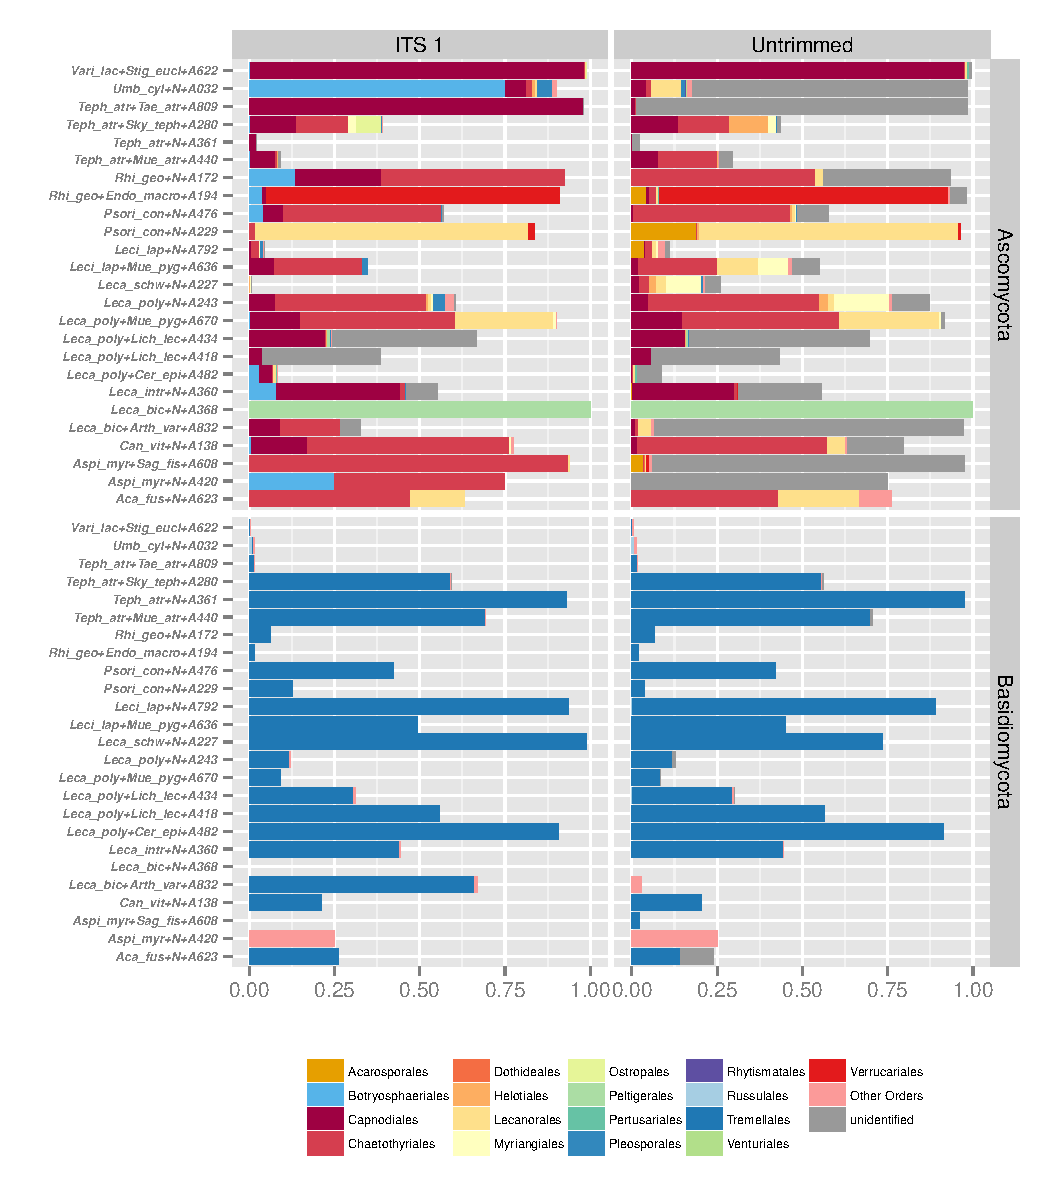
\includegraphics[width=\maxwidth]{figure/10_PlotOrders-1} \caption[Overview of Taxonomic composition at Order level split by dataset and Division]{Overview of Taxonomic composition at Order level split by dataset and Division.}\label{fig:10_PlotOrders}
\end{figure}


\end{knitrout}
%
% Tables Orders ITSX
%
% latex table generated in R 3.0.3 by xtable 1.7-4 package
% Tue Feb  7 12:20:01 2017
\begin{sidewaystable}[b]
\centering
\caption[Order ITS1 I]{Proportion of sequences asignable to Fungal Orders in the trimmed ITS1 dataset (Part I)} 
\begin{tabular}{rrrrrrrrrrrrrrrrrrr}
  \hline
 & \begin{sideways} Botryosphaeriales \end{sideways} & \begin{sideways} Candelariales \end{sideways} & \begin{sideways} Capnodiales \end{sideways} & \begin{sideways} Chaetothyriales \end{sideways} & \begin{sideways} Diaporthales \end{sideways} & \begin{sideways} Eurotiales \end{sideways} & \begin{sideways} Helotiales \end{sideways} & \begin{sideways} Hypocreales \end{sideways} & \begin{sideways} Lecanorales \end{sideways} & \begin{sideways} Lecideales \end{sideways} & \begin{sideways} Myriangiales \end{sideways} & \begin{sideways} Ostropales \end{sideways} & \begin{sideways} Peltigerales \end{sideways} & \begin{sideways} Pertusariales \end{sideways} & \begin{sideways} Pleosporales \end{sideways} & \begin{sideways} Rhizocarpales \end{sideways} & \begin{sideways} Saccharomycetales \end{sideways} & \begin{sideways} Taphrinales \end{sideways} \\ 
  \hline
Aca\_fus+N+A623 & . & . & . & 9 & . & . & . & . & 3 & . & . & . & . & . & . & . & . & . \\ 
  Aspi\_myr+N+A420 & 1 & . & . & 2 & . & . & . & . & . & . & . & . & . & . & . & . & . & . \\ 
  Aspi\_myr+Sag\_fis+A608 & . & . & 2 & 896 & . & . & . & . & 2 & . & . & . & . & . & . & . & . & . \\ 
  Can\_vit+N+A138 & 1 & . & 29 & 103 & . & . & . & . & . & . & 1 & . & . & . & . & 1 & . & . \\ 
  Leca\_bic+Arth\_var+A832 & . & . & 25 & 48 & . & . & . & . & . & . & . & . & . & . & . & . & . & . \\ 
  Leca\_bic+N+A368 & . & . & . & . & . & . & . & . & . & . & . & . & 16 & . & . & . & . & . \\ 
  Leca\_intr+N+A360 & 422 & . & 1900 & 76 & . & . & . & . & 1 & . & 1 & . & . & . & 3 & . & . & . \\ 
  Leca\_poly+Cer\_epi+A482 & 10 & 1 & 13 & 1 & . & . & . & . & 3 & . & . & . & . & 1 & . & . & . & . \\ 
  Leca\_poly+Lich\_lec+A418 & . & . & 2 & . & . & . & . & . & . & . & . & . & . & . & . & . & . & . \\ 
  Leca\_poly+Lich\_lec+A434 & . & . & 208 & 4 & . & . & 2 & 3 & . & . & . & . & 7 & . & 2 & . & . & . \\ 
  Leca\_poly+Mue\_pyg+A670 & 9 & . & 379 & 1178 & . & . & . & . & 745 & . & 17 & . & . & . & . & 1 & . & . \\ 
  Leca\_poly+N+A243 & 2 & 10 & 193 & 1125 & . & . & 16 & 59 & 19 & 1 & 17 & . & . & . & 89 & . & . & . \\ 
  Leca\_schw+N+A227 & 1 & . & 4 & 10 & . & . & 1 & . & 2 & . & 19 & 1 & . & . & 1 & . & . & . \\ 
  Leci\_lap+Mue\_pyg+A636 & . & . & 6 & 21 & . & . & . & . & . & . & . & . & . & . & 1 & . & . & . \\ 
  Leci\_lap+N+A792 & . & 1 & 6 & 20 & . & . & . & . & 2 & . & 1 & . & . & . & 9 & . & . & . \\ 
  Psori\_con+N+A229 & . & . & . & 1 & . & . & . & . & 44 & . & . & . & . & . & . & . & . & . \\ 
  Psori\_con+N+A476 & 21 & . & 27 & 224 & . & . & . & . & . & . & 1 & . & . & . & 1 & . & . & . \\ 
  Rhi\_geo+Endo\_macro+A194 & 44 & . & 11 & 1 & . & . & . & . & . & . & . & . & . & . & . & . & . & . \\ 
  Rhi\_geo+N+A172 & 24 & . & 44 & 94 & . & . & . & . & . & . & . & . & . & . & . & . & . & . \\ 
  Teph\_atr+Mue\_atr+A440 & 4 & . & 80 & 4 & . & . & 3 & . & . & . & . & . & . & . & . & . & . & . \\ 
  Teph\_atr+N+A361 & 9 & . & 121 & 1 & . & . & . & . & . & . & . & . & . & . & 2 & . & . & . \\ 
  Teph\_atr+Sky\_teph+A280 & 30 & . & 785 & 899 & . & 2 & . & . & . & . & 146 & 424 & . & . & 11 & 1 & . & 4 \\ 
  Teph\_atr+Tae\_atr+A809 & . & . & 5225 & 2 & . & . & . & . & . & . & . & . & . & . & 1 & . & . & . \\ 
  Umb\_cyl+N+A032 & 2063 & . & 169 & 49 & 6 & . & 22 & 11 & 14 & 7 & . & . & . & . & 120 & 7 & 1 & . \\ 
  Vari\_lac+Stig\_eucl+A622 & 14 & . & 2907 & 6 & . & . & . & . & 4 & . & . & 2 & . & . & . & . & . & . \\ 
   \hline
\end{tabular}
\end{sidewaystable}
% latex table generated in R 3.0.3 by xtable 1.7-4 package
% Tue Feb  7 12:20:01 2017
\begin{sidewaystable}[b]
\centering
\caption[Order ITS1 II]{Proportion of sequences asignable to Fungal Orders the trimmed ITS1 dataset (Part II)} 
\begin{tabular}{rrrrrrrrrrrrrrrr}
  \hline
 & \begin{sideways} Umbilicariales \end{sideways} & \begin{sideways} Verrucariales \end{sideways} & \begin{sideways} Agaricales \end{sideways} & \begin{sideways} Auriculariales \end{sideways} & \begin{sideways} Cantharellales \end{sideways} & \begin{sideways} Corticiales \end{sideways} & \begin{sideways} Cystofilobasidiales \end{sideways} & \begin{sideways} Hymenochaetales \end{sideways} & \begin{sideways} Polyporales \end{sideways} & \begin{sideways} Russulales \end{sideways} & \begin{sideways} Sebacinales \end{sideways} & \begin{sideways} Sporidiobolales \end{sideways} & \begin{sideways} Tremellales \end{sideways} & \begin{sideways} Blastocladiales \end{sideways} & \begin{sideways} unidentified \end{sideways} \\ 
  \hline
Aca\_fus+N+A623 & . & . & . & . & . & . & . & . & . & . & . & . & 5 & . & 2 \\ 
  Aspi\_myr+N+A420 & . & . & . & . & . & . & . & . & . & . & 1 & . & . & . & . \\ 
  Aspi\_myr+Sag\_fis+A608 & . & . & . & . & . & . & . & . & . & . & . & . & . & . & 58 \\ 
  Can\_vit+N+A138 & . & . & . & . & . & . & . & . & . & . & . & . & 37 & . & 2 \\ 
  Leca\_bic+Arth\_var+A832 & . & . & 2 & . & . & . & . & 1 & . & . & . & . & 180 & . & 17 \\ 
  Leca\_bic+N+A368 & . & . & . & . & . & . & . & . & . & . & . & . & . & . & . \\ 
  Leca\_intr+N+A360 & . & 1 & . & . & . & . & . & . & 1 & . & . & . & 2309 & . & 508 \\ 
  Leca\_poly+Cer\_epi+A482 & . & . & . & . & . & . & . & . & . & . & . & . & 311 & . & 3 \\ 
  Leca\_poly+Lich\_lec+A418 & . & . & . & . & . & . & . & . & . & . & . & . & 29 & . & 21 \\ 
  Leca\_poly+Lich\_lec+A434 & . & . & . & . & . & . & . & . & 5 & 2 & . & . & 282 & . & 414 \\ 
  Leca\_poly+Mue\_pyg+A670 & 1 & . & . & . & . & . & . & . & . & . & . & . & 237 & . & 21 \\ 
  Leca\_poly+N+A243 & . & . & . & . & . & . & . & . & . & 1 & . & 1 & 303 & . & 704 \\ 
  Leca\_schw+N+A227 & . & . & . & . & . & . & . & . & . & . & . & . & 6164 & . & 23 \\ 
  Leci\_lap+Mue\_pyg+A636 & . & . & . & . & . & . & . & . & . & . & . & . & 40 & . & 13 \\ 
  Leci\_lap+N+A792 & . & . & . & . & . & . & . & . & . & 1 & . & . & 835 & . & 17 \\ 
  Psori\_con+N+A229 & . & 1 & . & . & . & . & . & . & . & . & . & . & 7 & . & 2 \\ 
  Psori\_con+N+A476 & . & . & . & . & . & . & . & . & . & . & . & . & 205 & . & 4 \\ 
  Rhi\_geo+Endo\_macro+A194 & . & 952 & . & . & . & . & . & . & . & . & . & . & 19 & . & 80 \\ 
  Rhi\_geo+N+A172 & . & . & . & . & . & . & . & . & . & . & . & . & 11 & . & 2 \\ 
  Teph\_atr+Mue\_atr+A440 & 1 & . & . & . & 1 & . & . & . & . & . & . & . & 740 & . & 237 \\ 
  Teph\_atr+N+A361 & . & . & . & . & . & . & . & . & . & . & . & . & 5822 & . & 306 \\ 
  Teph\_atr+Sky\_teph+A280 & . & . & 6 & 2 & . & 1 & 4 & 1 & 3 & 2 & . & . & 3466 & . & 101 \\ 
  Teph\_atr+Tae\_atr+A809 & . & . & . & . & . & . & . & 1 & . & . & . & . & 87 & . & 14 \\ 
  Umb\_cyl+N+A032 & 1 & . & 5 & . & 3 & . & . & . & 6 & 24 & . & . & 7 & 1 & 228 \\ 
  Vari\_lac+Stig\_eucl+A622 & . & . & 1 & . & . & . & . & . & . & . & . & . & 10 & . & 24 \\ 
   \hline
\end{tabular}
\end{sidewaystable}

\newpage
%
% Tables Orders MEGAN
%
% latex table generated in R 3.0.3 by xtable 1.7-4 package
% Tue Feb  7 12:20:01 2017
\begin{sidewaystable}[b]
\centering
\caption[Orders MEGAN I]{Proportion of sequences asignable to Fungal Orders in the untrimmed dataset (Part I)} 
\begin{tabular}{rrrrrrrrrrrrrrrrrrr}
  \hline
 & \begin{sideways} Acarosporales \end{sideways} & \begin{sideways} Candelariales \end{sideways} & \begin{sideways} Capnodiales \end{sideways} & \begin{sideways} Chaetothyriales \end{sideways} & \begin{sideways} Diaporthales \end{sideways} & \begin{sideways} Dothideales \end{sideways} & \begin{sideways} Eurotiales \end{sideways} & \begin{sideways} Helotiales \end{sideways} & \begin{sideways} Hypocreales \end{sideways} & \begin{sideways} Lecanorales \end{sideways} & \begin{sideways} Lecideales \end{sideways} & \begin{sideways} Myriangiales \end{sideways} & \begin{sideways} Orbiliales \end{sideways} & \begin{sideways} Peltigerales \end{sideways} & \begin{sideways} Pertusariales \end{sideways} & \begin{sideways} Phacidiales \end{sideways} & \begin{sideways} Phaeomoniellales \end{sideways} & \begin{sideways} Pleosporales \end{sideways} \\ 
  \hline
Aca\_fus+N+A623 & . & . & . & 9 & . & . & . & . & . & 5 & . & . & . & . & . & . & . & . \\ 
  Aspi\_myr+N+A420 & . & . & . & . & . & . & . & . & . & . & . & . & . & . & . & . & . & . \\ 
  Aspi\_myr+Sag\_fis+A608 & 32 & . & . & 3 & . & 1 & . & . & . & 3 & . & . & . & . & . & . & . & . \\ 
  Can\_vit+N+A138 & . & . & 3 & 104 & . & . & . & . & . & 10 & . & . & . & . & . & . & . & . \\ 
  Leca\_bic+Arth\_var+A832 & . & . & 1 & 1 & . & . & . & . & . & 4 & . & . & . & . & . & . & . & . \\ 
  Leca\_bic+N+A368 & . & . & . & . & . & . & . & . & . & . & . & . & . & 16 & . & . & . & . \\ 
  Leca\_intr+N+A360 & 2 & . & 1610 & 40 & . & . & . & . & . & 7 & . & 1 & . & . & . & . & 1 & 2 \\ 
  Leca\_poly+Cer\_epi+A482 & . & . & 1 & 1 & . & . & . & . & . & 2 & . & . & . & . & 2 & . & . & . \\ 
  Leca\_poly+Lich\_lec+A418 & . & . & 3 & . & . & . & . & . & . & . & . & . & . & . & . & . & . & . \\ 
  Leca\_poly+Lich\_lec+A434 & . & . & 152 & . & . & . & . & 1 & . & . & . & . & . & 8 & . & . & . & 2 \\ 
  Leca\_poly+Mue\_pyg+A670 & . & . & 391 & 1213 & . & . & . & 6 & 1 & 769 & . & 17 & . & . & . & . & . & . \\ 
  Leca\_poly+N+A243 & . & . & 116 & 1232 & . & . & . & 69 & 2 & 42 & 1 & 394 & 9 & . & . & . & 9 & . \\ 
  Leca\_schw+N+A227 & . & 1 & 4 & 5 & . & . & . & 4 & . & 5 & . & 18 & . & . & . & . & . & 1 \\ 
  Leci\_lap+Mue\_pyg+A636 & . & . & 2 & 23 & . & . & . & . & . & 12 & . & 9 & . & . & . & . & 1 & . \\ 
  Leci\_lap+N+A792 & 36 & 14 & 2 & 20 & . & . & . & . & . & 13 & . & 6 & . & . & . & . & 2 & 1 \\ 
  Psori\_con+N+A229 & 36 & . & . & 1 & . & . & . & 1 & . & 145 & . & . & . & . & . & . & . & . \\ 
  Psori\_con+N+A476 & . & . & 3 & 231 & . & . & . & 2 & . & 5 & . & 1 & . & . & . & . & . & 1 \\ 
  Rhi\_geo+Endo\_macro+A194 & 45 & . & 11 & 21 & . & . & 5 & . & . & 6 & . & . & . & . & 2 & . & . & . \\ 
  Rhi\_geo+N+A172 & . & . & . & 98 & . & . & . & . & . & 4 & . & . & . & . & . & . & . & . \\ 
  Teph\_atr+Mue\_atr+A440 & . & . & 81 & 184 & . & . & . & 1 & . & . & . & . & . & . & . & . & . & . \\ 
  Teph\_atr+N+A361 & . & . & 17 & 1 & . & . & . & . & . & . & . & . & . & . & . & . & . & . \\ 
  Teph\_atr+Sky\_teph+A280 & 2 & 2 & 845 & 920 & . & . & 2 & 719 & . & 5 & . & 146 & . & . & . & . & . & 4 \\ 
  Teph\_atr+Tae\_atr+A809 & . & . & 59 & 10 & . & . & . & . & . & . & . & . & . & . & 1 & . & . & 1 \\ 
  Umb\_cyl+N+A032 & . & . & 119 & 40 & 6 & 1 & . & 1 & 1 & 246 & 7 & . & . & 1 & . & 9 & . & 35 \\ 
  Vari\_lac+Stig\_eucl+A622 & . & . & 3005 & 6 & . & . & . & 2 & . & 14 & . & . & . & . & 25 & . & . & . \\ 
   \hline
\end{tabular}
\end{sidewaystable}
% latex table generated in R 3.0.3 by xtable 1.7-4 package
% Tue Feb  7 12:20:01 2017
\begin{sidewaystable}[b]
\centering
\caption[Orders MEGAN II]{Proportion of sequences asignable to Fungal Orders in the untrimmed dataset  (Part II)} 
\begin{tabular}{rrrrrrrrrrrrrrrrrrrrrr}
  \hline
 & \begin{sideways} Rhizocarpales \end{sideways} & \begin{sideways} Rhytismatales \end{sideways} & \begin{sideways} Saccharomycetales \end{sideways} & \begin{sideways} Taphrinales \end{sideways} & \begin{sideways} Trapeliales \end{sideways} & \begin{sideways} Umbilicariales \end{sideways} & \begin{sideways} Venturiales \end{sideways} & \begin{sideways} Verrucariales \end{sideways} & \begin{sideways} Agaricales \end{sideways} & \begin{sideways} Auriculariales \end{sideways} & \begin{sideways} Corticiales \end{sideways} & \begin{sideways} Cystofilobasidiales \end{sideways} & \begin{sideways} Holtermanniales \end{sideways} & \begin{sideways} Hymenochaetales \end{sideways} & \begin{sideways} Malasseziales \end{sideways} & \begin{sideways} Polyporales \end{sideways} & \begin{sideways} Russulales \end{sideways} & \begin{sideways} Sebacinales \end{sideways} & \begin{sideways} Tremellales \end{sideways} & \begin{sideways} Blastocladiales \end{sideways} & \begin{sideways} Unknown \end{sideways} \\ 
  \hline
Aca\_fus+N+A623 & 2 & . & . & . & . & . & . & . & . & . & . & . & . & . & . & . & . & . & 3 & . & 2 \\ 
  Aspi\_myr+N+A420 & . & . & . & . & . & . & . & . & . & . & . & . & . & . & . & . & . & 1 & . & . & 3 \\ 
  Aspi\_myr+Sag\_fis+A608 & . & . & . & . & . & 9 & . & 8 & . & . & . & . & . & . & . & . & . & . & 22 & . & 856 \\ 
  Can\_vit+N+A138 & 1 & . & . & . & . & . & . & . & . & . & . & . & . & . & . & . & . & . & 38 & . & 31 \\ 
  Leca\_bic+Arth\_var+A832 & . & . & . & . & . & 1 & . & . & 2 & . & . & . & . & 1 & . & . & . & . & . & . & 96 \\ 
  Leca\_bic+N+A368 & . & . & . & . & . & . & . & . & . & . & . & . & . & . & . & . & . & . & . & . & . \\ 
  Leca\_intr+N+A360 & 1 & . & . & . & . & . & . & 1 & . & . & . & . & . & . & . & 1 & . & . & 2373 & . & 1304 \\ 
  Leca\_poly+Cer\_epi+A482 & . & . & . & . & . & . & . & . & . & . & . & . & . & . & . & . & . & . & 321 & . & 24 \\ 
  Leca\_poly+Lich\_lec+A418 & . & . & . & . & . & . & . & . & . & . & . & . & . & . & . & . & . & . & 30 & . & 20 \\ 
  Leca\_poly+Lich\_lec+A434 & . & . & . & . & . & 1 & . & . & . & . & . & . & . & . & . & 5 & 2 & . & 283 & . & 509 \\ 
  Leca\_poly+Mue\_pyg+A670 & 1 & . & . & . & . & 3 & . & . & . & . & . & . & . & . & . & . & . & . & 222 & . & 18 \\ 
  Leca\_poly+N+A243 & . & . & . & . & . & . & 1 & 1 & . & . & . & . & . & 1 & . & . & . & . & 292 & . & 284 \\ 
  Leca\_schw+N+A227 & . & . & . & . & . & . & . & . & . & . & . & . & . & . & . & . & . & . & 130 & . & 9 \\ 
  Leci\_lap+Mue\_pyg+A636 & . & . & . & . & . & . & . & . & . & . & . & . & . & . & . & . & . & . & 45 & . & 8 \\ 
  Leci\_lap+N+A792 & . & . & . & . & . & 2 & . & . & . & . & . & . & . & . & . & . & 1 & . & 872 & . & 13 \\ 
  Psori\_con+N+A229 & . & . & . & . & . & . & . & 1 & . & . & . & . & . & . & . & . & . & . & 7 & . & . \\ 
  Psori\_con+N+A476 & . & . & . & . & . & . & . & . & . & . & . & . & . & . & . & . & . & . & 212 & . & 47 \\ 
  Rhi\_geo+Endo\_macro+A194 & . & . & . & . & . & 1 & . & 895 & . & . & . & . & . & . & . & . & . & . & 19 & . & 50 \\ 
  Rhi\_geo+N+A172 & . & . & . & . & . & . & . & . & . & . & . & . & . & . & . & . & . & . & 12 & . & 68 \\ 
  Teph\_atr+Mue\_atr+A440 & 1 & . & . & . & . & 1 & . & 2 & . & . & . & . & . & . & . & . & . & . & 734 & . & 47 \\ 
  Teph\_atr+N+A361 & . & . & . & . & . & . & . & . & . & . & . & . & . & . & . & . & . & . & 5821 & . & 124 \\ 
  Teph\_atr+Sky\_teph+A280 & 1 & . & . & 5 & 2 & 2 & . & . & 7 & 2 & 2 & 4 & . & . & 1 & 4 & 2 & . & 3448 & . & 74 \\ 
  Teph\_atr+Tae\_atr+A809 & . & . & . & . & . & . & . & . & . & . & . & . & . & 1 & . & . & . & . & 88 & . & 5540 \\ 
  Umb\_cyl+N+A032 & 14 & 12 & 2 & . & . & 2 & 8 & . & 5 & . & 3 & . & 1 & . & . & 6 & 25 & . & . & 2 & 2271 \\ 
  Vari\_lac+Stig\_eucl+A622 & . & . & . & . & . & . & . & . & 1 & . & . & . & . & . & . & . & . & . & 10 & . & 18 \\ 
   \hline
\end{tabular}
\end{sidewaystable}

\subsection{Families}
%
% PLOT OF FAMILY ASCRIPTION
%
\begin{knitrout}
\definecolor{shadecolor}{rgb}{0.969, 0.969, 0.969}\color{fgcolor}\begin{figure}[H]
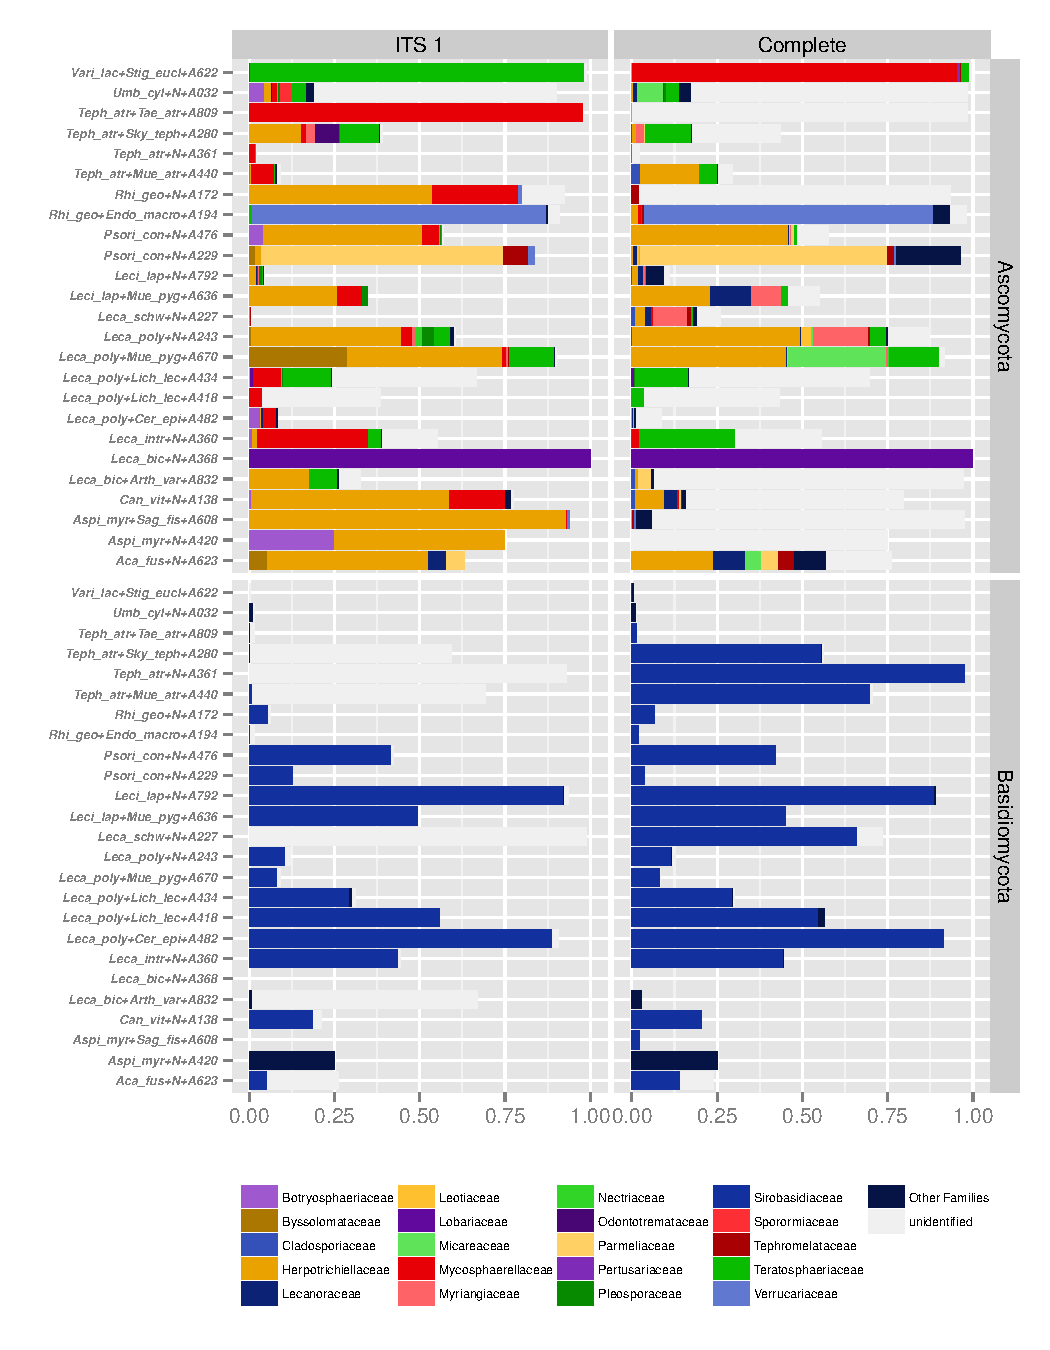
\includegraphics[width=\maxwidth]{figure/14_PlotFamilies-1} \caption[Overview of Taxonomic composition at Family level split by dataset and Division]{Overview of Taxonomic composition at Family level split by dataset and Division. Minoritary Families within Asco and Basidiomycota were recoded as "other" for graphical simplicity. Full Results can be found in tables X:Y}\label{fig:14_PlotFamilies}
\end{figure}


\end{knitrout}
%<<14_PlotFamilieslegend, echo=FALSE, fig.height=4, fig.width=4, fig.pos='H'>>=
%plot(g_legend(mof))
%@
\newpage
%
% TABLE FAMILIES ITS1
%
% latex table generated in R 3.0.3 by xtable 1.7-4 package
% Tue Feb  7 12:20:03 2017
\begin{sidewaystable}[b]
\centering
\caption[Families ITS1 I]{Proportion of sequences asignable to Fungal Families the trimmed ITS1 dataset (Part I)} 
\begin{tabular}{rrrrrrrrrrrrrrrrrrr}
  \hline
 & \begin{sideways} Botryosphaeriaceae \end{sideways} & \begin{sideways} Byssolomataceae \end{sideways} & \begin{sideways} Candelariaceae \end{sideways} & \begin{sideways} Catenariaceae \end{sideways} & \begin{sideways} Chaetothyriaceae \end{sideways} & \begin{sideways} Chionosphaeraceae \end{sideways} & \begin{sideways} Corticiaceae \end{sideways} & \begin{sideways} Cystofilobasidiaceae \end{sideways} & \begin{sideways} Davidiellaceae \end{sideways} & \begin{sideways} Dermateaceae \end{sideways} & \begin{sideways} Filobasidiaceae \end{sideways} & \begin{sideways} Fomitopsidaceae \end{sideways} & \begin{sideways} Ganodermataceae \end{sideways} & \begin{sideways} Helotiaceae \end{sideways} & \begin{sideways} Hemiphacidiaceae \end{sideways} & \begin{sideways} Herpotrichiellaceae \end{sideways} & \begin{sideways} Hyaloscyphaceae \end{sideways} & \begin{sideways} Hydnaceae \end{sideways} \\ 
  \hline
Aca\_fus+N+A623 & . & 1 & . & . & . & . & . & . & . & . & . & . & . & . & . & 9 & . & . \\ 
  Aspi\_myr+N+A420 & 1 & . & . & . & . & . & . & . & . & . & . & . & . & . & . & 2 & . & . \\ 
  Aspi\_myr+Sag\_fis+A608 & . & . & . & . & . & . & . & . & . & . & . & . & . & . & . & 891 & . & . \\ 
  Can\_vit+N+A138 & 1 & . & . & . & 2 & . & . & . & . & . & . & . & . & . & . & 101 & . & . \\ 
  Leca\_bic+Arth\_var+A832 & . & . & . & . & . & . & . & . & 1 & . & . & . & . & . & . & 48 & . & . \\ 
  Leca\_bic+N+A368 & . & . & . & . & . & . & . & . & . & . & . & . & . & . & . & . & . & . \\ 
  Leca\_intr+N+A360 & 53 & . & . & . & . & . & . & . & 4 & . & . & . & . & . & . & 77 & . & . \\ 
  Leca\_poly+Cer\_epi+A482 & 10 & 1 & 1 & . & . & . & . & . & . & . & . & . & . & . & . & 1 & . & . \\ 
  Leca\_poly+Lich\_lec+A418 & . & . & . & . & . & . & . & . & . & . & . & . & . & . & . & . & . & . \\ 
  Leca\_poly+Lich\_lec+A434 & . & . & . & . & . & . & . & . & . & . & . & . & . & . & 1 & 4 & . & . \\ 
  Leca\_poly+Mue\_pyg+A670 & . & 744 & . & . & . & . & . & . & . & . & . & . & . & . & . & 1178 & . & . \\ 
  Leca\_poly+N+A243 & . & 14 & 10 & . & . & 1 & . & . & 1 & 8 & 2 & . & . & . & . & 1122 & 7 & . \\ 
  Leca\_schw+N+A227 & . & . & . & . & . & . & . & . & 2 & . & . & . & . & . & . & 10 & . & . \\ 
  Leci\_lap+Mue\_pyg+A636 & . & . & . & . & . & . & . & . & . & . & . & . & . & . & . & 21 & . & . \\ 
  Leci\_lap+N+A792 & . & . & 1 & . & . & . & . & . & 1 & . & . & . & . & . & . & 20 & . & . \\ 
  Psori\_con+N+A229 & . & 1 & . & . & . & . & . & . & . & . & . & . & . & . & . & 1 & . & . \\ 
  Psori\_con+N+A476 & 21 & . & . & . & . & . & . & . & . & . & . & . & . & . & . & 224 & . & . \\ 
  Rhi\_geo+Endo\_macro+A194 & . & . & . & . & . & . & . & . & . & . & . & . & . & . & . & 1 & . & . \\ 
  Rhi\_geo+N+A172 & . & . & . & . & . & . & . & . & . & . & . & . & . & . & . & 94 & . & . \\ 
  Teph\_atr+Mue\_atr+A440 & 4 & . & . & . & . & . & . & . & 1 & . & . & . & . & . & . & 4 & 3 & . \\ 
  Teph\_atr+N+A361 & 6 & . & . & . & . & . & . & . & 1 & . & . & . & . & . & . & 1 & . & . \\ 
  Teph\_atr+Sky\_teph+A280 & 1 & . & . & . & . & . & 1 & 4 & 5 & . & . & . & . & . & . & 897 & . & . \\ 
  Teph\_atr+Tae\_atr+A809 & . & . & . & . & . & . & . & . & . & . & . & . & . & . & . & 2 & . & . \\ 
  Umb\_cyl+N+A032 & 127 & . & . & 1 & . & . & . & . & . & . & . & 1 & 3 & 1 & 12 & 49 & . & 3 \\ 
  Vari\_lac+Stig\_eucl+A622 & . & . & . & . & . & . & . & . & 1 & . & . & . & . & . & . & 3 & . & . \\ 
   \hline
\end{tabular}
\end{sidewaystable}
% latex table generated in R 3.0.3 by xtable 1.7-4 package
% Tue Feb  7 12:20:03 2017
\begin{sidewaystable}[b]
\centering
\caption[Families ITS1 II]{Proportion of sequences asignable to Fungal Families the trimmed ITS1 dataset (Part II)} 
\begin{tabular}{rrrrrrrrrrrrrrrrrrrr}
  \hline
 & \begin{sideways} Hymenochaetaceae \end{sideways} & \begin{sideways} Lecanoraceae \end{sideways} & \begin{sideways} Lecideaceae \end{sideways} & \begin{sideways} Leptosphaeriaceae \end{sideways} & \begin{sideways} Lobariaceae \end{sideways} & \begin{sideways} Marasmiaceae \end{sideways} & \begin{sideways} Megasporaceae \end{sideways} & \begin{sideways} Melanommataceae \end{sideways} & \begin{sideways} Meruliaceae \end{sideways} & \begin{sideways} Mycenaceae \end{sideways} & \begin{sideways} Mycosphaerellaceae \end{sideways} & \begin{sideways} Myriangiaceae \end{sideways} & \begin{sideways} Nectriaceae \end{sideways} & \begin{sideways} Odontotremataceae \end{sideways} & \begin{sideways} Ophiocordycipitaceae \end{sideways} & \begin{sideways} Ophioparmaceae \end{sideways} & \begin{sideways} Parmeliaceae \end{sideways} & \begin{sideways} Peniophoraceae \end{sideways} & \begin{sideways} Phacidiaceae \end{sideways} \\ 
  \hline
Aca\_fus+N+A623 & . & 1 & . & . & . & . & . & . & . & . & . & . & . & . & . & . & 1 & . & . \\ 
  Aspi\_myr+N+A420 & . & . & . & . & . & . & . & . & . & . & . & . & . & . & . & . & . & . & . \\ 
  Aspi\_myr+Sag\_fis+A608 & . & . & . & . & . & . & . & . & . & . & 2 & . & . & . & . & . & . & . & . \\ 
  Can\_vit+N+A138 & . & . & . & . & . & . & . & . & . & . & 29 & . & . & . & . & . & . & . & . \\ 
  Leca\_bic+Arth\_var+A832 & 1 & . & . & . & . & 2 & . & . & . & . & . & . & . & . & . & . & . & . & . \\ 
  Leca\_bic+N+A368 & . & . & . & . & 16 & . & . & . & . & . & . & . & . & . & . & . & . & . & . \\ 
  Leca\_intr+N+A360 & . & . & . & 1 & . & . & . & . & . & . & 1694 & 1 & . & . & . & . & 1 & . & . \\ 
  Leca\_poly+Cer\_epi+A482 & . & 2 & . & . & . & . & 1 & . & . & . & 13 & . & . & . & . & . & . & . & . \\ 
  Leca\_poly+Lich\_lec+A418 & . & . & . & . & . & . & . & . & . & . & 2 & . & . & . & . & . & . & . & . \\ 
  Leca\_poly+Lich\_lec+A434 & . & . & . & . & 7 & . & . & . & 2 & . & 77 & . & 3 & . & . & . & . & 2 & . \\ 
  Leca\_poly+Mue\_pyg+A670 & . & . & . & . & . & . & . & . & . & . & 32 & 17 & . & . & . & . & . & . & . \\ 
  Leca\_poly+N+A243 & . & 1 & 1 & . & . & . & . & 1 & . & . & 81 & 17 & 57 & . & 2 & . & 1 & 1 & . \\ 
  Leca\_schw+N+A227 & . & 1 & . & . & . & . & . & . & . & . & 1 & 19 & . & 1 & . & . & . & . & . \\ 
  Leci\_lap+Mue\_pyg+A636 & . & . & . & . & . & . & . & . & . & . & 6 & . & . & . & . & . & . & . & . \\ 
  Leci\_lap+N+A792 & . & 1 & . & . & . & . & . & . & . & . & 4 & 1 & . & . & . & . & 1 & 1 & . \\ 
  Psori\_con+N+A229 & . & . & . & . & . & . & . & . & . & . & . & . & . & . & . & . & 39 & . & . \\ 
  Psori\_con+N+A476 & . & . & . & . & . & . & . & . & . & . & 25 & 1 & . & . & . & . & . & . & . \\ 
  Rhi\_geo+Endo\_macro+A194 & . & . & . & . & . & . & 8 & . & . & . & . & . & . & . & . & . & . & . & . \\ 
  Rhi\_geo+N+A172 & . & . & . & . & . & . & . & . & . & . & 44 & . & . & . & . & . & . & . & . \\ 
  Teph\_atr+Mue\_atr+A440 & . & . & . & . & . & . & . & . & . & . & 71 & . & . & . & . & . & . & . & . \\ 
  Teph\_atr+N+A361 & . & . & . & . & . & . & . & . & . & . & 112 & . & . & . & . & . & . & . & . \\ 
  Teph\_atr+Sky\_teph+A280 & . & . & . & . & . & 1 & . & . & 2 & 1 & 96 & 146 & . & 424 & . & . & . & 2 & . \\ 
  Teph\_atr+Tae\_atr+A809 & . & . & . & . & . & . & . & . & . & . & 5222 & . & . & . & . & . & . & . & . \\ 
  Umb\_cyl+N+A032 & . & 13 & 7 & . & . & . & . & 16 & . & . & 38 & . & 11 & . & . & 1 & 1 & . & 9 \\ 
  Vari\_lac+Stig\_eucl+A622 & . & 3 & . & . & . & . & . & . & . & . & 6 & . & . & 2 & . & . & 1 & . & . \\ 
   \hline
\end{tabular}
\end{sidewaystable}
% latex table generated in R 3.0.3 by xtable 1.7-4 package
% Tue Feb  7 12:20:03 2017
\begin{sidewaystable}[b]
\centering
\caption[Families ITS1 III]{Proportion of sequences asignable to Fungal Families the trimmed ITS1 dataset (Part III)} 
\begin{tabular}{rrrrrrrrrrrrrrrrrr}
  \hline
 & \begin{sideways} Phaeosphaeriaceae \end{sideways} & \begin{sideways} Physalacriaceae \end{sideways} & \begin{sideways} Pleosporaceae \end{sideways} & \begin{sideways} Pleurotaceae \end{sideways} & \begin{sideways} Polyporaceae \end{sideways} & \begin{sideways} Psathyrellaceae \end{sideways} & \begin{sideways} Rhizocarpaceae \end{sideways} & \begin{sideways} Schizoporaceae \end{sideways} & \begin{sideways} Sclerotiniaceae \end{sideways} & \begin{sideways} Sebacinaceae \end{sideways} & \begin{sideways} Sirobasidiaceae \end{sideways} & \begin{sideways} Sporormiaceae \end{sideways} & \begin{sideways} Stereaceae \end{sideways} & \begin{sideways} Strophariaceae \end{sideways} & \begin{sideways} Taphrinaceae \end{sideways} & \begin{sideways} Tephromelataceae \end{sideways} & \begin{sideways} Teratosphaeriaceae \end{sideways} \\ 
  \hline
Aca\_fus+N+A623 & . & . & . & . & . & . & . & . & . & . & 1 & . & . & . & . & . & . \\ 
  Aspi\_myr+N+A420 & . & . & . & . & . & . & . & . & . & 1 & . & . & . & . & . & . & . \\ 
  Aspi\_myr+Sag\_fis+A608 & . & . & . & . & . & . & . & . & . & . & . & . & . & . & . & 2 & . \\ 
  Can\_vit+N+A138 & . & . & . & . & . & . & 1 & . & . & . & 33 & . & . & . & . & . & . \\ 
  Leca\_bic+Arth\_var+A832 & . & . & . & . & . & . & . & . & . & . & . & . & . & . & . & . & 23 \\ 
  Leca\_bic+N+A368 & . & . & . & . & . & . & . & . & . & . & . & . & . & . & . & . & . \\ 
  Leca\_intr+N+A360 & . & . & . & . & 1 & . & . & . & . & . & 2284 & 2 & . & . & . & . & 201 \\ 
  Leca\_poly+Cer\_epi+A482 & . & . & . & . & . & . & . & . & . & . & 305 & . & . & . & . & . & . \\ 
  Leca\_poly+Lich\_lec+A418 & . & . & . & . & . & . & . & . & . & . & 29 & . & . & . & . & . & . \\ 
  Leca\_poly+Lich\_lec+A434 & . & . & 2 & . & 3 & . & . & . & . & . & 274 & . & . & . & . & . & 131 \\ 
  Leca\_poly+Mue\_pyg+A670 & . & . & . & . & . & . & 1 & . & . & . & 217 & . & . & . & . & 1 & 347 \\ 
  Leca\_poly+N+A243 & 1 & . & 87 & . & . & . & . & . & . & . & 270 & . & . & . & . & 3 & 113 \\ 
  Leca\_schw+N+A227 & . & . & . & . & . & . & . & . & 1 & . & 9 & 1 & . & . & . & 1 & 1 \\ 
  Leci\_lap+Mue\_pyg+A636 & . & . & 1 & . & . & . & . & . & . & . & 40 & . & . & . & . & . & . \\ 
  Leci\_lap+N+A792 & . & . & 9 & . & . & . & . & . & . & . & 823 & . & . & . & . & . & 1 \\ 
  Psori\_con+N+A229 & . & . & . & . & . & . & . & . & . & . & 7 & . & . & . & . & 4 & . \\ 
  Psori\_con+N+A476 & . & . & 1 & . & . & . & . & . & . & . & 202 & . & . & . & . & . & 2 \\ 
  Rhi\_geo+Endo\_macro+A194 & . & . & . & . & . & . & . & . & . & . & 3 & . & . & . & . & . & 11 \\ 
  Rhi\_geo+N+A172 & . & . & . & . & . & . & . & . & . & . & 10 & . & . & . & . & . & . \\ 
  Teph\_atr+Mue\_atr+A440 & . & . & . & . & . & . & . & . & . & . & 9 & . & . & . & . & . & 5 \\ 
  Teph\_atr+N+A361 & . & . & 2 & . & . & . & . & . & . & . & 9 & . & . & . & . & . & 8 \\ 
  Teph\_atr+Sky\_teph+A280 & . & 2 & 10 & . & 1 & 1 & 1 & 1 & . & 2 & 2 & . & . & . & 4 & . & 683 \\ 
  Teph\_atr+Tae\_atr+A809 & . & . & 1 & . & . & . & . & 1 & . & . & 13 & . & . & . & . & . & 3 \\ 
  Umb\_cyl+N+A032 & . & . & 16 & 2 & 2 & 3 & 7 & . & . & . & . & 82 & 24 & . & . & . & 125 \\ 
  Vari\_lac+Stig\_eucl+A622 & . & . & . & . & . & . & . & . & . & . & . & . & . & 1 & . & . & 2900 \\ 
   \hline
\end{tabular}
\end{sidewaystable}
% latex table generated in R 3.0.3 by xtable 1.7-4 package
% Tue Feb  7 12:20:03 2017
\begin{sidewaystable}[b]
\centering
\caption[Families ITS1 IV]{Proportion of sequences asignable to Fungal Families the trimmed ITS1 dataset (Part IV)} 
\begin{tabular}{rrrrrrrrr}
  \hline
 & \begin{sideways} Thelebolaceae \end{sideways} & \begin{sideways} Trichocomaceae \end{sideways} & \begin{sideways} Tricholomataceae \end{sideways} & \begin{sideways} Umbilicariaceae \end{sideways} & \begin{sideways} unidentified \end{sideways} & \begin{sideways} Valsaceae \end{sideways} & \begin{sideways} Venturiaceae \end{sideways} & \begin{sideways} Verrucariaceae \end{sideways} \\ 
  \hline
Aca\_fus+N+A623 & . & . & . & . & 6 & . & . & . \\ 
  Aspi\_myr+N+A420 & . & . & . & . & . & . & . & . \\ 
  Aspi\_myr+Sag\_fis+A608 & . & . & . & . & 58 & . & . & 5 \\ 
  Can\_vit+N+A138 & . & . & . & . & 7 & . & . & . \\ 
  Leca\_bic+Arth\_var+A832 & . & . & . & . & 198 & . & . & . \\ 
  Leca\_bic+N+A368 & . & . & . & . & . & . & . & . \\ 
  Leca\_intr+N+A360 & . & . & . & . & 902 & . & . & 1 \\ 
  Leca\_poly+Cer\_epi+A482 & . & . & . & . & 9 & . & . & . \\ 
  Leca\_poly+Lich\_lec+A418 & . & . & . & . & 21 & . & . & . \\ 
  Leca\_poly+Lich\_lec+A434 & 1 & . & . & . & 422 & . & . & . \\ 
  Leca\_poly+Mue\_pyg+A670 & . & . & . & 1 & 50 & . & . & . \\ 
  Leca\_poly+N+A243 & . & . & . & . & 738 & . & 1 & . \\ 
  Leca\_schw+N+A227 & . & . & . & . & 6179 & . & . & . \\ 
  Leci\_lap+Mue\_pyg+A636 & . & . & . & . & 13 & . & . & . \\ 
  Leci\_lap+N+A792 & . & . & . & . & 29 & . & . & . \\ 
  Psori\_con+N+A229 & . & . & . & . & 2 & . & . & 1 \\ 
  Psori\_con+N+A476 & . & . & . & . & 7 & . & . & . \\ 
  Rhi\_geo+Endo\_macro+A194 & . & . & . & . & 132 & . & . & 952 \\ 
  Rhi\_geo+N+A172 & . & . & . & . & 25 & . & . & 2 \\ 
  Teph\_atr+Mue\_atr+A440 & . & . & . & 1 & 972 & . & . & . \\ 
  Teph\_atr+N+A361 & . & . & . & . & 6122 & . & . & . \\ 
  Teph\_atr+Sky\_teph+A280 & . & 2 & 1 & . & 3597 & 1 & . & . \\ 
  Teph\_atr+Tae\_atr+A809 & . & . & . & . & 88 & . & . & . \\ 
  Umb\_cyl+N+A032 & . & . & . & 1 & 2177 & 6 & 6 & . \\ 
  Vari\_lac+Stig\_eucl+A622 & . & . & . & . & 51 & . & . & . \\ 
   \hline
\end{tabular}
\end{sidewaystable}

\newpage
%
% TABLE FAMILIES MEGAN
%
% latex table generated in R 3.0.3 by xtable 1.7-4 package
% Tue Feb  7 12:20:04 2017
\begin{sidewaystable}[b]
\centering
\caption[Families ITS1 I]{Proportion of sequences asignable to Fungal Families in the untrimmed dataset (Part I)} 
\begin{tabular}{rrrrrrrrrrrrrrrrrrr}
  \hline
 & \begin{sideways} Acarosporaceae \end{sideways} & \begin{sideways} Agaricaceae \end{sideways} & \begin{sideways} Aspergillaceae \end{sideways} & \begin{sideways} Candelariaceae \end{sideways} & \begin{sideways} Catenariaceae \end{sideways} & \begin{sideways} Cladoniaceae \end{sideways} & \begin{sideways} Cladosporiaceae \end{sideways} & \begin{sideways} Coriolaceae \end{sideways} & \begin{sideways} Corticiaceae \end{sideways} & \begin{sideways} Cortinariaceae \end{sideways} & \begin{sideways} Cyphellophoraceae \end{sideways} & \begin{sideways} Cystofilobasidiaceae \end{sideways} & \begin{sideways} Didymellaceae \end{sideways} & \begin{sideways} Dothioraceae \end{sideways} & \begin{sideways} Exidiaceae \end{sideways} & \begin{sideways} Ganodermataceae \end{sideways} & \begin{sideways} Helotiaceae \end{sideways} & \begin{sideways} Hemiphacidiaceae \end{sideways} \\ 
  \hline
Aca\_fus+N+A623 & . & . & . & . & . & . & . & . & . & . & . & . & . & . & . & . & . & . \\ 
  Aspi\_myr+N+A420 & . & . & . & . & . & . & . & . & . & . & . & . & . & . & . & . & . & . \\ 
  Aspi\_myr+Sag\_fis+A608 & 32 & . & . & . & . & . & . & . & . & . & . & . & . & 1 & . & . & . & . \\ 
  Can\_vit+N+A138 & . & . & . & . & . & 1 & 2 & . & . & . & . & . & . & . & . & . & . & . \\ 
  Leca\_bic+Arth\_var+A832 & . & . & . & . & . & . & 1 & . & . & . & . & . & . & . & . & . & . & . \\ 
  Leca\_bic+N+A368 & . & . & . & . & . & . & . & . & . & . & . & . & . & . & . & . & . & . \\ 
  Leca\_intr+N+A360 & 2 & . & . & . & . & . & 4 & . & . & . & . & . & . & . & . & . & . & . \\ 
  Leca\_poly+Cer\_epi+A482 & . & . & . & . & . & . & . & . & . & . & . & . & . & . & . & . & . & . \\ 
  Leca\_poly+Lich\_lec+A418 & . & . & . & . & . & . & . & . & . & . & . & . & . & . & . & . & . & . \\ 
  Leca\_poly+Lich\_lec+A434 & . & . & . & . & . & . & . & 1 & . & . & . & . & . & . & . & . & . & 1 \\ 
  Leca\_poly+Mue\_pyg+A670 & . & . & . & . & . & . & . & . & . & . & . & . & . & . & . & . & . & . \\ 
  Leca\_poly+N+A243 & . & . & . & . & . & . & 1 & . & . & . & . & . & . & . & . & . & . & . \\ 
  Leca\_schw+N+A227 & . & . & . & 1 & . & . & 2 & . & . & . & . & . & . & . & . & . & . & . \\ 
  Leci\_lap+Mue\_pyg+A636 & . & . & . & . & . & . & . & . & . & . & . & . & . & . & . & . & . & . \\ 
  Leci\_lap+N+A792 & 36 & . & . & 14 & . & . & 1 & . & . & . & . & . & . & . & . & . & . & . \\ 
  Psori\_con+N+A229 & 36 & . & . & . & . & . & . & . & . & . & . & . & . & . & . & . & . & . \\ 
  Psori\_con+N+A476 & . & . & . & . & . & . & . & . & . & . & . & . & . & . & . & . & . & . \\ 
  Rhi\_geo+Endo\_macro+A194 & 45 & . & 5 & . & . & . & . & . & . & . & . & . & . & . & . & . & . & . \\ 
  Rhi\_geo+N+A172 & . & . & . & . & . & . & . & . & . & . & . & . & . & . & . & . & . & . \\ 
  Teph\_atr+Mue\_atr+A440 & . & . & . & . & . & . & 27 & . & . & . & 1 & . & . & . & . & . & . & . \\ 
  Teph\_atr+N+A361 & . & . & . & . & . & . & 1 & . & . & . & . & . & . & . & . & . & . & . \\ 
  Teph\_atr+Sky\_teph+A280 & 2 & 1 & 2 & 2 & . & . & 6 & 2 & 1 & . & . & 4 & 2 & . & 2 & . & . & . \\ 
  Teph\_atr+Tae\_atr+A809 & . & . & . & . & . & . & . & . & . & . & . & . & . & . & . & . & . & . \\ 
  Umb\_cyl+N+A032 & . & . & . & . & 2 & . & . & 3 & 3 & . & . & . & . & . & . & 3 & 1 & . \\ 
  Vari\_lac+Stig\_eucl+A622 & . & . & . & . & . & . & 1 & . & . & 1 & . & . & . & . & . & . & . & . \\ 
   \hline
\end{tabular}
\end{sidewaystable}
% latex table generated in R 3.0.3 by xtable 1.7-4 package
% Tue Feb  7 12:20:04 2017
\begin{sidewaystable}[b]
\centering
\caption[Families ITS1 II]{Proportion of sequences asignable to Fungal Families in the untrimmed dataset (Part II)} 
\begin{tabular}{rrrrrrrrrrrrrrrrrrrr}
  \hline
 & \begin{sideways} Herpotrichiellaceae \end{sideways} & \begin{sideways} Hymenochaetaceae \end{sideways} & \begin{sideways} Lecanoraceae \end{sideways} & \begin{sideways} Lecideaceae \end{sideways} & \begin{sideways} Leotiaceae \end{sideways} & \begin{sideways} Lobariaceae \end{sideways} & \begin{sideways} Malasseziaceae \end{sideways} & \begin{sideways} Marasmiaceae \end{sideways} & \begin{sideways} Megasporaceae \end{sideways} & \begin{sideways} Melanommataceae \end{sideways} & \begin{sideways} Meruliaceae \end{sideways} & \begin{sideways} Micareaceae \end{sideways} & \begin{sideways} Mycosphaerellaceae \end{sideways} & \begin{sideways} Myriangiaceae \end{sideways} & \begin{sideways} Nectriaceae \end{sideways} & \begin{sideways} Ophiocordycipitaceae \end{sideways} & \begin{sideways} Ophioparmaceae \end{sideways} & \begin{sideways} Orbiliaceae \end{sideways} & \begin{sideways} Parmeliaceae \end{sideways} \\ 
  \hline
Aca\_fus+N+A623 & 5 & . & 2 & . & . & . & . & . & . & . & . & 1 & . & . & . & . & . & . & 1 \\ 
  Aspi\_myr+N+A420 & . & . & . & . & . & . & . & . & . & . & . & . & . & . & . & . & . & . & . \\ 
  Aspi\_myr+Sag\_fis+A608 & 3 & . & . & . & . & . & . & . & . & . & . & . & . & . & . & . & . & . & . \\ 
  Can\_vit+N+A138 & 16 & . & 7 & . & . & . & . & . & . & . & . & . & 1 & . & . & . & . & . & 1 \\ 
  Leca\_bic+Arth\_var+A832 & 1 & 1 & . & . & . & . & . & . & . & . & . & . & . & . & . & . & . & . & 4 \\ 
  Leca\_bic+N+A368 & . & . & . & . & . & 16 & . & . & . & . & . & . & . & . & . & . & . & . & . \\ 
  Leca\_intr+N+A360 & 9 & . & . & . & . & . & . & . & . & . & . & . & 102 & 1 & . & . & . & . & 1 \\ 
  Leca\_poly+Cer\_epi+A482 & 1 & . & 1 & . & . & . & . & . & 2 & . & . & 1 & . & . & . & . & . & . & . \\ 
  Leca\_poly+Lich\_lec+A418 & . & . & . & . & . & . & . & . & . & . & . & . & . & . & . & . & . & . & . \\ 
  Leca\_poly+Lich\_lec+A434 & . & . & . & . & . & 8 & . & . & . & . & 2 & . & . & . & . & . & . & . & . \\ 
  Leca\_poly+Mue\_pyg+A670 & 1195 & . & 11 & . & 6 & . & . & . & . & . & . & 757 & 4 & 17 & 1 & . & . & . & . \\ 
  Leca\_poly+N+A243 & 1209 & 1 & 12 & 1 & 69 & . & . & . & . & . & . & 15 & . & 394 & . & 2 & . & 9 & 2 \\ 
  Leca\_schw+N+A227 & 5 & . & 3 & . & . & . & . & . & . & . & . & . & 1 & 18 & . & . & . & . & . \\ 
  Leci\_lap+Mue\_pyg+A636 & 23 & . & 12 & . & . & . & . & . & . & . & . & . & . & 9 & . & . & . & . & . \\ 
  Leci\_lap+N+A792 & 19 & . & 13 & . & . & . & . & . & . & . & . & . & . & 6 & . & . & . & . & . \\ 
  Psori\_con+N+A229 & 1 & . & 2 & . & 1 & . & . & . & . & . & . & 1 & . & . & . & . & . & . & 138 \\ 
  Psori\_con+N+A476 & 231 & . & 1 & . & 2 & . & . & . & . & . & . & . & . & 1 & . & . & . & . & 4 \\ 
  Rhi\_geo+Endo\_macro+A194 & 20 & . & . & . & . & . & . & . & . & . & . & . & 10 & . & . & . & . & . & . \\ 
  Rhi\_geo+N+A172 & . & . & . & . & . & . & . & . & . & . & . & . & . & . & . & . & . & . & . \\ 
  Teph\_atr+Mue\_atr+A440 & 181 & . & . & . & 1 & . & . & . & . & . & . & . & . & . & . & . & . & . & . \\ 
  Teph\_atr+N+A361 & . & . & . & . & . & . & . & . & . & . & . & . & . & . & . & . & . & . & . \\ 
  Teph\_atr+Sky\_teph+A280 & 80 & . & 2 & . & . & . & 1 & 1 & . & . & 2 & . & 3 & 146 & . & . & . & . & 3 \\ 
  Teph\_atr+Tae\_atr+A809 & 8 & . & . & . & . & . & . & . & . & . & . & . & . & . & . & . & . & . & . \\ 
  Umb\_cyl+N+A032 & 17 & . & 29 & 7 & . & 1 & . & . & . & 19 & . & 212 & 10 & . & 1 & . & 1 & . & . \\ 
  Vari\_lac+Stig\_eucl+A622 & 2 & . & 7 & . & . & . & . & . & . & . & . & . & 2934 & . & . & . & . & . & . \\ 
   \hline
\end{tabular}
\end{sidewaystable}
% latex table generated in R 3.0.3 by xtable 1.7-4 package
% Tue Feb  7 12:20:04 2017
\begin{sidewaystable}[b]
\centering
\caption[Families ITS1 III]{Proportion of sequences asignable to Fungal Families in the untrimmed  dataset (Part III)} 
\begin{tabular}{rrrrrrrrrrrrrrrrrr}
  \hline
 & \begin{sideways} Peniophoraceae \end{sideways} & \begin{sideways} Pertusariaceae \end{sideways} & \begin{sideways} Phacidiaceae \end{sideways} & \begin{sideways} Physalacriaceae \end{sideways} & \begin{sideways} Pleosporaceae \end{sideways} & \begin{sideways} Pleurotaceae \end{sideways} & \begin{sideways} Polyporaceae \end{sideways} & \begin{sideways} Psathyrellaceae \end{sideways} & \begin{sideways} Pseudoperisporiaceae \end{sideways} & \begin{sideways} Rhizocarpaceae \end{sideways} & \begin{sideways} Rhytismataceae \end{sideways} & \begin{sideways} Rutstroemiaceae \end{sideways} & \begin{sideways} Sebacinaceae \end{sideways} & \begin{sideways} Sirobasidiaceae \end{sideways} & \begin{sideways} Sporormiaceae \end{sideways} & \begin{sideways} Stereaceae \end{sideways} & \begin{sideways} Sympoventuriaceae \end{sideways} \\ 
  \hline
Aca\_fus+N+A623 & . & . & . & . & . & . & . & . & . & 2 & . & . & . & 3 & . & . & . \\ 
  Aspi\_myr+N+A420 & . & . & . & . & . & . & . & . & . & . & . & . & 1 & . & . & . & . \\ 
  Aspi\_myr+Sag\_fis+A608 & . & . & . & . & . & . & . & . & . & . & . & . & . & 22 & . & . & . \\ 
  Can\_vit+N+A138 & . & . & . & . & . & . & . & . & . & 1 & . & . & . & 38 & . & . & . \\ 
  Leca\_bic+Arth\_var+A832 & . & . & . & . & . & . & . & . & . & . & . & . & . & . & . & . & . \\ 
  Leca\_bic+N+A368 & . & . & . & . & . & . & . & . & . & . & . & . & . & . & . & . & . \\ 
  Leca\_intr+N+A360 & . & . & . & . & . & . & 1 & . & . & 1 & . & . & . & 2373 & 2 & . & . \\ 
  Leca\_poly+Cer\_epi+A482 & . & . & . & . & . & . & . & . & . & . & . & . & . & 321 & . & . & . \\ 
  Leca\_poly+Lich\_lec+A418 & . & . & . & . & . & . & . & . & . & . & . & . & . & 29 & . & . & . \\ 
  Leca\_poly+Lich\_lec+A434 & 2 & . & . & . & 2 & . & . & . & . & . & . & . & . & 283 & . & . & . \\ 
  Leca\_poly+Mue\_pyg+A670 & . & . & . & . & . & . & . & . & . & 1 & . & . & . & 220 & . & . & . \\ 
  Leca\_poly+N+A243 & . & . & . & . & . & . & . & . & . & . & . & . & . & 282 & . & . & . \\ 
  Leca\_schw+N+A227 & . & . & . & . & . & . & . & . & . & . & . & 1 & . & 117 & . & . & . \\ 
  Leci\_lap+Mue\_pyg+A636 & . & . & . & . & . & . & . & . & . & . & . & . & . & 45 & . & . & . \\ 
  Leci\_lap+N+A792 & 1 & . & . & . & 1 & . & . & . & . & . & . & . & . & 872 & . & . & . \\ 
  Psori\_con+N+A229 & . & . & . & . & . & . & . & . & . & . & . & . & . & 7 & . & . & . \\ 
  Psori\_con+N+A476 & . & . & . & . & 1 & . & . & . & . & . & . & . & . & 212 & . & . & . \\ 
  Rhi\_geo+Endo\_macro+A194 & . & 2 & . & . & . & . & . & . & . & . & . & . & . & 19 & . & . & . \\ 
  Rhi\_geo+N+A172 & . & . & . & . & . & . & . & . & . & . & . & . & . & 12 & . & . & . \\ 
  Teph\_atr+Mue\_atr+A440 & . & . & . & . & . & . & . & . & . & 1 & . & . & . & 734 & . & . & . \\ 
  Teph\_atr+N+A361 & . & . & . & . & . & . & . & . & . & . & . & . & . & 5821 & . & . & . \\ 
  Teph\_atr+Sky\_teph+A280 & 2 & . & . & 2 & 2 & . & . & . & . & 1 & . & . & . & 3444 & . & . & . \\ 
  Teph\_atr+Tae\_atr+A809 & . & 1 & . & . & 1 & . & . & . & . & . & . & . & . & 88 & . & . & . \\ 
  Umb\_cyl+N+A032 & . & . & 9 & . & 16 & 2 & . & 3 & 20 & 14 & 12 & . & . & . & . & 25 & 1 \\ 
  Vari\_lac+Stig\_eucl+A622 & . & 25 & . & . & . & . & . & . & . & . & . & . & . & 10 & . & . & . \\ 
   \hline
\end{tabular}
\end{sidewaystable}
% latex table generated in R 3.0.3 by xtable 1.7-4 package
% Tue Feb  7 12:20:04 2017
\begin{sidewaystable}[b]
\centering
\caption[Families ITS1 IV]{Proportion of sequences asignable to Fungal Families in the untrimmed  dataset (Part IV)} 
\begin{tabular}{rrrrrrrrrrrrr}
  \hline
 & \begin{sideways} Taphrinaceae \end{sideways} & \begin{sideways} Tephromelataceae \end{sideways} & \begin{sideways} Teratosphaeriaceae \end{sideways} & \begin{sideways} Trapeliaceae \end{sideways} & \begin{sideways} Tremellaceae \end{sideways} & \begin{sideways} Tricholomataceae \end{sideways} & \begin{sideways} Umbilicariaceae \end{sideways} & \begin{sideways} Unknown \end{sideways} & \begin{sideways} Valsaceae \end{sideways} & \begin{sideways} Venturiaceae \end{sideways} & \begin{sideways} Verrucariaceae \end{sideways} & \begin{sideways} Vuilleminiaceae \end{sideways} \\ 
  \hline
Aca\_fus+N+A623 & . & 1 & . & . & . & . & . & 6 & . & . & . & . \\ 
  Aspi\_myr+N+A420 & . & . & . & . & . & . & . & 3 & . & . & . & . \\ 
  Aspi\_myr+Sag\_fis+A608 & . & 3 & . & . & . & . & 9 & 856 & . & . & 8 & . \\ 
  Can\_vit+N+A138 & . & 1 & . & . & . & . & . & 119 & . & . & . & . \\ 
  Leca\_bic+Arth\_var+A832 & . & . & . & . & . & 2 & 1 & 96 & . & . & . & . \\ 
  Leca\_bic+N+A368 & . & . & . & . & . & . & . & . & . & . & . & . \\ 
  Leca\_intr+N+A360 & . & 6 & 1495 & . & . & . & . & 1345 & . & . & 1 & . \\ 
  Leca\_poly+Cer\_epi+A482 & . & . & . & . & . & . & . & 25 & . & . & . & . \\ 
  Leca\_poly+Lich\_lec+A418 & . & . & 2 & . & 1 & . & . & 21 & . & . & . & . \\ 
  Leca\_poly+Lich\_lec+A434 & . & . & 150 & . & . & . & 1 & 513 & . & . & . & . \\ 
  Leca\_poly+Mue\_pyg+A670 & . & 1 & 386 & . & 2 & . & 3 & 37 & . & . & . & . \\ 
  Leca\_poly+N+A243 & . & 13 & 114 & . & 10 & . & . & 317 & . & 1 & 1 & . \\ 
  Leca\_schw+N+A227 & . & 2 & 1 & . & . & . & . & 26 & . & . & . & . \\ 
  Leci\_lap+Mue\_pyg+A636 & . & . & 2 & . & . & . & . & 9 & . & . & . & . \\ 
  Leci\_lap+N+A792 & . & . & 1 & . & . & . & 2 & 16 & . & . & . & . \\ 
  Psori\_con+N+A229 & . & 4 & . & . & . & . & . & . & . & . & 1 & . \\ 
  Psori\_con+N+A476 & . & . & 3 & . & . & . & . & 47 & . & . & . & . \\ 
  Rhi\_geo+Endo\_macro+A194 & . & 6 & 1 & . & . & . & 1 & 51 & . & . & 895 & . \\ 
  Rhi\_geo+N+A172 & . & 4 & . & . & . & . & . & 166 & . & . & . & . \\ 
  Teph\_atr+Mue\_atr+A440 & . & . & 54 & . & . & . & 1 & 49 & . & . & 2 & . \\ 
  Teph\_atr+N+A361 & . & . & 14 & . & . & . & . & 127 & . & . & . & . \\ 
  Teph\_atr+Sky\_teph+A280 & 5 & . & 836 & 2 & 1 & 3 & 2 & 1636 & . & . & . & 1 \\ 
  Teph\_atr+Tae\_atr+A809 & . & . & . & . & . & . & . & 5602 & . & . & . & . \\ 
  Umb\_cyl+N+A032 & . & . & 108 & . & . & . & 1 & 2284 & 6 & 7 & . & . \\ 
  Vari\_lac+Stig\_eucl+A622 & . & 7 & 70 & . & . & . & . & 24 & . & . & . & . \\ 
   \hline
\end{tabular}
\end{sidewaystable}

\newpage
\section{Diversity Patterns}
\subsection{OTU Diversity and rarefaction curves}
\begin{knitrout}
\definecolor{shadecolor}{rgb}{0.969, 0.969, 0.969}\color{fgcolor}\begin{figure}[H]
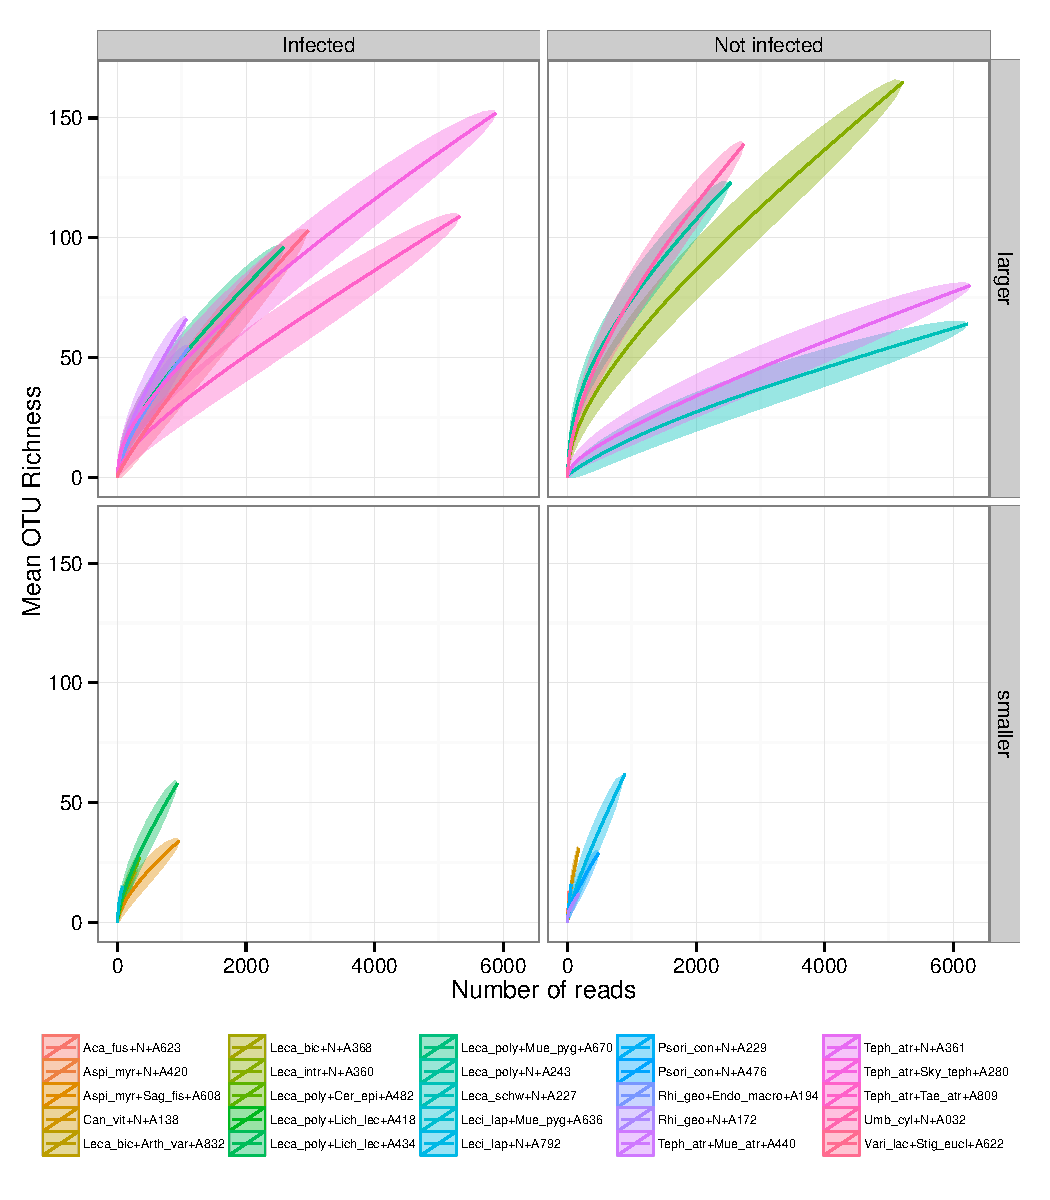
\includegraphics[width=\maxwidth]{figure/rarefact-1} \caption[Rarefaction curves of OTU richness per samples]{Rarefaction curves of OTU richness per samples. All singletons were included.}\label{fig:rarefact}
\end{figure}


\end{knitrout}
%
%<<rarefact1a, echo=FALSE, message=FALSE, error=FALSE, warning=FALSE, fig.height=8, fig.pos='H', fig.lp="fig:", fig.cap='Average rarefied OTU Richness per treatment. All singletons were included.'>>=
%#
%# ERASE PDF INSERT FOR CULOPOLLO
%#
%#
%#pdf("/Users/ferninfm/Dropbox/ANTONIA/3_Paper/Material_for_figures/alpha_Z.pdf")
%#alpha.n<-alpha$richness[,c(1,2,4,6,7,12,13,15,16,17,19,21,24)]
%#alpha.i<-alpha$richness[,-c(1,2,4,6,7,12,13,15,16,17,19,21,24)]
%#SE.n<-alpha$SE[,c(1,2,4,6,7,12,13,15,16,17,19,21,24)]
%#SE.n<-sqrt(rowSums(SE.n^2))
%#SE.i<-alpha$SE[,-c(1,2,4,6,7,12,13,15,16,17,19,21,24)]
%#SE.i<-sqrt(rowSums(SE.i^2))
%#counts.n<-rowSums(!is.na(alpha.n))
%#counts.i<-rowSums(!is.na(alpha.i))
%#alpha.n<-rowMeans(alpha.n,na.rm=T)
%#alpha.i<-rowMeans(alpha.i,na.rm=T)
%#
%#
%alpha.plot<-data.frame(rbind(cbind(alpha.n,alpha.n-(1.96*SE.n),alpha.n+(1.96*SE.n),as.numeric(alpha$subsample),0),cbind(alpha.i,alpha.i-(1.96*SE.i),alpha.i+(1.96*SE.i),as.numeric(alpha$subsample),1)))
%names(alpha.plot)<-c("alpha","cilow","cihigh","sequences","treatment")
%alpha.plot<-alpha.plot[-c(131:134),]
%p.alpha<-ggplot(alpha.plot,aes(x=as.numeric(sequences), y=as.numeric(alpha), ymin=as.numeric(cilow), ymax=as.numeric(cihigh), fill=as.factor(treatment), colour=as.factor(treatment)))
%print(p.alpha+geom_point()+geom_errorbar())
%#+ facet_wrap(~ treatment) + scale_fill_manual(values=c("#E69F00", "#56B4E9")))
%#
%# P on the difference of the means
%#
%#
%z.test<-mat.or.vec(length(alpha.n),2)
%for (i in 1:length(alpha.n))
%{
%z.test[i,1]<-(alpha.n[i]-alpha.i[i])/sqrt(
%(((SE.n[i]^2)/counts.n[i])+((SE.i[i]^2)/counts.i[i])))
%z.test[i,2]<-2*pnorm(-abs(z.test[i,1]))
%}
%z.test<-data.frame(z.test)
%z.test<-cbind(z.test,as.numeric(alpha$subsample))#$
%names(z.test)<-c("X1","X2","X3")
%z.test<-z.test[-c(1,64,65,66,67),]
%p.z<-ggplot(data=z.test,aes(x=X3, y=X1, fill=as.factor((z.test[,2]<=0.05)), colour=as.factor((z.test[,2]<=0.05))))
%print(p.z+geom_point())
%dev.off()
%@




%
% FERNANDO
%
%
%<<rarefact2, echo=FALSE, message=FALSE, error=FALSE, warning=FALSE, fig.height=8, fig.pos='H', fig.lp="fig:", fig.cap='Rarefaction curves of OTU richness per samples. All singletons were excluded.'>>=
%library(reshape2)
%otu.table<-tabulate.and.print(data=seq.subset, samples=1, groups=5, normalize=FALSE, print=FALSE)
%otu.table[[1]]<-otu.table[[1]][,order(as.numeric(colnames(otu.table[[1]])))]
%otu.table[[1]]<-otu.table[[1]][,colSums(otu.table[[1]])!=1]
%alpha<-rarefaction(otu.table[[1]],subsample=150)
%#
%#
%# PLOT RESULTS
%#
%#
%# Dataframe to ggplot
%dc<-cbind(melt(alpha$richness),melt(alpha$SE))[,c(3,1,2,5)]
%colnames(dc)<-c("rarefy","sample","metric","SE")
%dc<-dc[!is.na(dc$metric),]
%variable.treatment<-as.matrix(dc$sample)
%variable.treatment[-(grep("+N+",variable.treatment))]<-"Infected"
%variable.treatment[grep("+N+",variable.treatment)]<-"Not infected"
%ciMult <- qt(0.95/2 + .5, 9) #datac$N-1)
%dc<-cbind(dc,factor(variable.treatment),dc$metric+(ciMult*dc$SE),dc$metric-(ciMult*dc$SE))#$
%colnames(dc)[5:7]<-c("treatment","ci.min","ci.max")
%# ggplot
%pd <- position_dodge(0.1)
%hulls<-rbind(dc[,c(1,2,5,6)],setNames(dc[length(dc[,1]):1,c(1,2,5,7)],names(dc[,c(1,2,5,6)])))
%#
%#
%#
%# Make Dummy Variable for plotting
%#
%#
%#
%element<-as.matrix(hulls[,2])
%element[element=="Aspi_myr+N+A420"]<-"smaller"
%element[element=="Leca_bic+N+A368"]<-"smaller"
%element[element=="Aca_fus+N+A623"]<-"smaller"
%element[element=="Psori_con+N+A229"]<-"smaller"
%element[element=="Can_vit+N+A138"]<-"smaller"
%element[element=="Rhi_geo+N+A172"]<-"smaller"
%element[element=="Leci_lap+Mue_pyg+A636"]<-"smaller"
%element[element=="Leca_poly+Lich_lec+A418"]<-"smaller"
%element[element=="Leca_bic+Arth_var+A832"]<-"smaller"
%element[element=="Leca_poly+Cer_epi+A482"]<-"smaller"
%element[element=="Leca_poly+Lich_lec+A434"]<-"smaller"
%element[element=="Aspi_myr+Sag_fis+A608"]<-"smaller"
%element[element=="Psori_con+N+A476"]<-"smaller"
%element[element=="Leci_lap+N+A792"]<-"smaller"
%element[element=="Leca_poly+N+A243"]<-"larger"
%element[element=="Umb_cyl+N+A032"]<-"larger"
%element[element=="Leca_intr+N+A360"]<-"larger"
%element[element=="Leca_schw+N+A227"]<-"larger"
%element[element=="Teph_atr+N+A361"]<-"larger"
%element[element=="Teph_atr+Mue_atr+A440"]<-"larger"
%element[element=="Rhi_geo+Endo_macro+A194"]<-"larger"
%element[element=="Leca_poly+Mue_pyg+A670"]<-"larger"
%element[element=="Vari_lac+Stig_eucl+A622"]<-"larger"
%element[element=="Teph_atr+Tae_atr+A809"]<-"larger"
%element[element=="Teph_atr+Sky_teph+A280"]<-"larger"
%hulls<-cbind(hulls,"sub.set"=element)
%#
%element<-as.matrix(dc[,2])
%element[element=="Aspi_myr+N+A420"]<-"smaller"
%element[element=="Leca_bic+N+A368"]<-"smaller"
%element[element=="Aca_fus+N+A623"]<-"smaller"
%element[element=="Psori_con+N+A229"]<-"smaller"
%element[element=="Can_vit+N+A138"]<-"smaller"
%element[element=="Rhi_geo+N+A172"]<-"smaller"
%element[element=="Leci_lap+Mue_pyg+A636"]<-"smaller"
%element[element=="Leca_poly+Lich_lec+A418"]<-"smaller"
%element[element=="Leca_bic+Arth_var+A832"]<-"smaller"
%element[element=="Leca_poly+Cer_epi+A482"]<-"smaller"
%element[element=="Leca_poly+Lich_lec+A434"]<-"smaller"
%element[element=="Aspi_myr+Sag_fis+A608"]<-"smaller"
%element[element=="Psori_con+N+A476"]<-"smaller"
%element[element=="Leci_lap+N+A792"]<-"smaller"
%element[element=="Leca_poly+N+A243"]<-"larger"
%element[element=="Umb_cyl+N+A032"]<-"larger"
%element[element=="Leca_intr+N+A360"]<-"larger"
%element[element=="Leca_schw+N+A227"]<-"larger"
%element[element=="Teph_atr+N+A361"]<-"larger"
%element[element=="Teph_atr+Mue_atr+A440"]<-"larger"
%element[element=="Rhi_geo+Endo_macro+A194"]<-"larger"
%element[element=="Leca_poly+Mue_pyg+A670"]<-"larger"
%element[element=="Vari_lac+Stig_eucl+A622"]<-"larger"
%element[element=="Teph_atr+Tae_atr+A809"]<-"larger"
%element[element=="Teph_atr+Sky_teph+A280"]<-"larger"
%dc<-cbind(dc,"sub.set"=element)
%#
%#
%#
%p1<-ggplot(dc,aes(x=rarefy, y=metric, fill=sample, colour=sample))
%#p1<-p1 + geom_errorbar(data=dc,aes(ymin=ci.min, ymax=ci.max), width=.25, position=pd)
%p1<-p1 + geom_polygon(data=hulls,
%	aes(
%		y=ci.min,
%			x=rarefy,
%			order=rownames(data),
%				fill=sample,
%				colour=NULL),
%				width=0.5,
%				position="identity",
%				alpha=0.4)
%p1<-p1 + geom_line(data=dc,aes(x=rarefy, y=metric, fill=NULL, colour=sample), position=pd)
%#p1<-p1 + geom_point(position=pd)
%p1<-p1 + labs (x="Number of reads", y="Mean OTU Richness") + theme_bw() + theme(
%			legend.box="horizontal",
%			legend.position="bottom",
%			legend.title=element_blank(),
%			legend.text=element_text(size=6),
%			legend.key.height=unit(0.16,"inch"),
%			legend.text=element_text(size=8))
%p1<-p1 + guides(fill=guide_legend(ncol=6))
%p1<-p1 + facet_grid(sub.set~treatment) 		
%print(p1)
%@
%<<rarefact2a, echo=FALSE, message=FALSE, error=FALSE, warning=FALSE, fig.height=8, fig.pos='H', fig.lp="fig:", fig.cap='Average rarefied OTU Richness per treatment. All singletons were excluded.'>>=
%#
%#
%#
%alpha.n<-alpha$richness[,c(1,2,4,6,7,12,13,15,16,17,19,21,24)]
%alpha.i<-alpha$richness[,-c(1,2,4,6,7,12,13,15,16,17,19,21,24)]
%SE.n<-alpha$SE[,c(1,2,4,6,7,12,13,15,16,17,19,21,24)]
%SE.n<-sqrt(rowSums(SE.n^2))
%SE.i<-alpha$SE[,-c(1,2,4,6,7,12,13,15,16,17,19,21,24)]
%SE.i<-sqrt(rowSums(SE.i^2))
%counts.n<-rowSums(!is.na(alpha.n))
%counts.i<-rowSums(!is.na(alpha.i))
%alpha.n<-rowMeans(alpha.n,na.rm=T)
%alpha.i<-rowMeans(alpha.i,na.rm=T)
%#
%#
%alpha.plot<-data.frame(rbind(cbind(alpha.n,alpha.n-(1.96*SE.n),alpha.n+(1.96*SE.n),as.numeric(alpha$subsample),0),cbind(alpha.i,alpha.i-(1.96*SE.i),alpha.i+(1.96*SE.i),as.numeric(alpha$subsample),1)))
%names(alpha.plot)<-c("alpha","cilow","cihigh","sequences","treatment")
%alpha.plot<-alpha.plot[-c(131:134),]
%p.alpha<-ggplot(alpha.plot,aes(x=as.numeric(sequences), y=as.numeric(alpha), ymin=as.numeric(cilow), ymax=as.numeric(cihigh), fill=as.factor(treatment), colour=as.factor(treatment)))
%print(p.alpha+geom_point()+geom_errorbar())
%#+ facet_wrap(~ treatment) + scale_fill_manual(values=c("#E69F00", "#56B4E9")))
%#
%# P on the difference of the means
%#
%#
%z.test<-mat.or.vec(length(alpha.n),2)
%for (i in 1:length(alpha.n))
%{
%z.test[i,1]<-(alpha.n[i]-alpha.i[i])/sqrt(
%(((SE.n[i]^2)/counts.n[i])+((SE.i[i]^2)/counts.i[i])))
%z.test[i,2]<-2*pnorm(-abs(z.test[i,1]))
%}
%z.test<-data.frame(z.test)
%z.test<-cbind(z.test,as.numeric(alpha$subsample))#$
%names(z.test)<-c("X1","X2","X3")
%z.test<-z.test[-c(1,64,65,66,67),]
%p.z<-ggplot(data=z.test,aes(x=X3, y=X1, fill=as.factor((z.test[,2]<=0.05)), colour=as.factor((z.test[,2]<=0.05))))
%print(p.z+geom_point())
%#dev.off()
%@
%
%\subsection{Taxonomic Diversity and rarefaction curves}
%
%At Order level
%
%<<rarefact_Orders, echo=FALSE, message=FALSE, error=FALSE, warning=FALSE, fig.height=8, fig.pos='H', fig.lp="fig:", fig.cap='Rarefaction curves of Taxonomic richness at Order level per sample'>>=
%otu.table<-tabulate.and.print(data=seq.subset, samples=1, groups=19, normalize=FALSE, print=FALSE)
%alpha<-rarefaction(otu.table[[1]],subsample=150)
%#
%#
%# PLOT RESULTS
%#
%#
%# Dataframe to ggplot
%dc<-cbind(melt(alpha$richness),melt(alpha$SE))[,c(3,1,2,5)]
%colnames(dc)<-c("rarefy","sample","metric","SE")
%dc<-dc[!is.na(dc$metric),]
%variable.treatment<-as.matrix(dc$sample)
%variable.treatment[-(grep("+N+",variable.treatment))]<-"Infected"
%variable.treatment[grep("+N+",variable.treatment)]<-"Not infected"
%ciMult <- qt(0.95/2 + .5, 9) #datac$N-1)
%dc<-cbind(dc,factor(variable.treatment),dc$metric+(ciMult*dc$SE),dc$metric-(ciMult*dc$SE))#$
%colnames(dc)[5:7]<-c("treatment","ci.min","ci.max")
%# ggplot
%pd <- position_dodge(0.1)
%hulls<-rbind(dc[,c(1,2,5,6)],setNames(dc[length(dc[,1]):1,c(1,2,5,7)],names(dc[,c(1,2,5,6)])))
%#
%#
%#
%# Make Dummy Variable for plotting
%#
%#
%#
%element<-as.matrix(hulls[,2])
%element[element=="Aspi_myr+N+A420"]<-"smaller"
%element[element=="Leca_bic+N+A368"]<-"smaller"
%element[element=="Aca_fus+N+A623"]<-"smaller"
%element[element=="Psori_con+N+A229"]<-"smaller"
%element[element=="Can_vit+N+A138"]<-"smaller"
%element[element=="Rhi_geo+N+A172"]<-"smaller"
%element[element=="Leci_lap+Mue_pyg+A636"]<-"smaller"
%element[element=="Leca_poly+Lich_lec+A418"]<-"smaller"
%element[element=="Leca_bic+Arth_var+A832"]<-"smaller"
%element[element=="Leca_poly+Cer_epi+A482"]<-"smaller"
%element[element=="Leca_poly+Lich_lec+A434"]<-"smaller"
%element[element=="Aspi_myr+Sag_fis+A608"]<-"smaller"
%element[element=="Psori_con+N+A476"]<-"smaller"
%element[element=="Leci_lap+N+A792"]<-"smaller"
%element[element=="Leca_poly+N+A243"]<-"larger"
%element[element=="Umb_cyl+N+A032"]<-"larger"
%element[element=="Leca_intr+N+A360"]<-"larger"
%element[element=="Leca_schw+N+A227"]<-"larger"
%element[element=="Teph_atr+N+A361"]<-"larger"
%element[element=="Teph_atr+Mue_atr+A440"]<-"larger"
%element[element=="Rhi_geo+Endo_macro+A194"]<-"larger"
%element[element=="Leca_poly+Mue_pyg+A670"]<-"larger"
%element[element=="Vari_lac+Stig_eucl+A622"]<-"larger"
%element[element=="Teph_atr+Tae_atr+A809"]<-"larger"
%element[element=="Teph_atr+Sky_teph+A280"]<-"larger"
%hulls<-cbind(hulls,"sub.set"=element)
%#
%element<-as.matrix(dc[,2])
%element[element=="Aspi_myr+N+A420"]<-"smaller"
%element[element=="Leca_bic+N+A368"]<-"smaller"
%element[element=="Aca_fus+N+A623"]<-"smaller"
%element[element=="Psori_con+N+A229"]<-"smaller"
%element[element=="Can_vit+N+A138"]<-"smaller"
%element[element=="Rhi_geo+N+A172"]<-"smaller"
%element[element=="Leci_lap+Mue_pyg+A636"]<-"smaller"
%element[element=="Leca_poly+Lich_lec+A418"]<-"smaller"
%element[element=="Leca_bic+Arth_var+A832"]<-"smaller"
%element[element=="Leca_poly+Cer_epi+A482"]<-"smaller"
%element[element=="Leca_poly+Lich_lec+A434"]<-"smaller"
%element[element=="Aspi_myr+Sag_fis+A608"]<-"smaller"
%element[element=="Psori_con+N+A476"]<-"smaller"
%element[element=="Leci_lap+N+A792"]<-"smaller"
%element[element=="Leca_poly+N+A243"]<-"larger"
%element[element=="Umb_cyl+N+A032"]<-"larger"
%element[element=="Leca_intr+N+A360"]<-"larger"
%element[element=="Leca_schw+N+A227"]<-"larger"
%element[element=="Teph_atr+N+A361"]<-"larger"
%element[element=="Teph_atr+Mue_atr+A440"]<-"larger"
%element[element=="Rhi_geo+Endo_macro+A194"]<-"larger"
%element[element=="Leca_poly+Mue_pyg+A670"]<-"larger"
%element[element=="Vari_lac+Stig_eucl+A622"]<-"larger"
%element[element=="Teph_atr+Tae_atr+A809"]<-"larger"
%element[element=="Teph_atr+Sky_teph+A280"]<-"larger"
%dc<-cbind(dc,"sub.set"=element)
%#
%#
%#
%p1<-ggplot(dc,aes(x=rarefy, y=metric, fill=sample, colour=sample))
%#p1<-p1 + geom_errorbar(data=dc,aes(ymin=ci.min, ymax=ci.max), width=.25, position=pd)
%p1<-p1 + geom_polygon(data=hulls,
%	aes(
%		y=ci.min,
%			x=rarefy,
%			order=rownames(data),
%				fill=sample,
%				colour=NULL),
%				width=0.5,
%				position="identity",
%				alpha=0.4)
%p1<-p1 + geom_line(data=dc,aes(x=rarefy, y=metric, fill=NULL, colour=sample), position=pd)
%#p1<-p1 + geom_point(position=pd)
%p1<-p1 + labs (x="Number of reads", y="Mean taxnonomic Richness") + theme_bw() + theme(
%			legend.box="horizontal",
%			legend.position="bottom",
%			legend.title=element_blank(),
%			legend.text=element_text(size=6),
%			legend.key.height=unit(0.16,"inch"),
%			legend.text=element_text(size=8))
%p1<-p1 + guides(fill=guide_legend(ncol=6))
%p1<-p1 + facet_grid(sub.set~treatment) 		
%print(p1)
%@
%
%<<rarefact_Families, echo=FALSE, message=FALSE, error=FALSE, warning=FALSE, fig.height=8, fig.pos='H', fig.lp="fig:", fig.cap='Rarefaction curves of Taxonomic richness at Family level per sample'>>=
%otu.table<-tabulate.and.print(data=seq.subset, samples=1, groups=21, normalize=FALSE, print=FALSE)
%alpha<-rarefaction(otu.table[[1]],subsample=150)
%#
%#
%# PLOT RESULTS
%#
%#
%# Dataframe to ggplot
%dc<-cbind(melt(alpha$richness),melt(alpha$SE))[,c(3,1,2,5)]
%colnames(dc)<-c("rarefy","sample","metric","SE")
%dc<-dc[!is.na(dc$metric),]
%variable.treatment<-as.matrix(dc$sample)
%variable.treatment[-(grep("+N+",variable.treatment))]<-"Infected"
%variable.treatment[grep("+N+",variable.treatment)]<-"Not infected"
%ciMult <- qt(0.95/2 + .5, 9) #datac$N-1)
%dc<-cbind(dc,factor(variable.treatment),dc$metric+(ciMult*dc$SE),dc$metric-(ciMult*dc$SE))#$
%colnames(dc)[5:7]<-c("treatment","ci.min","ci.max")
%# ggplot
%pd <- position_dodge(0.1)
%hulls<-rbind(dc[,c(1,2,5,6)],setNames(dc[length(dc[,1]):1,c(1,2,5,7)],names(dc[,c(1,2,5,6)])))
%#
%#
%#
%# Make Dummy Variable for plotting
%#
%#
%#
%element<-as.matrix(hulls[,2])
%element[element=="Aspi_myr+N+A420"]<-"smaller"
%element[element=="Leca_bic+N+A368"]<-"smaller"
%element[element=="Aca_fus+N+A623"]<-"smaller"
%element[element=="Psori_con+N+A229"]<-"smaller"
%element[element=="Can_vit+N+A138"]<-"smaller"
%element[element=="Rhi_geo+N+A172"]<-"smaller"
%element[element=="Leci_lap+Mue_pyg+A636"]<-"smaller"
%element[element=="Leca_poly+Lich_lec+A418"]<-"smaller"
%element[element=="Leca_bic+Arth_var+A832"]<-"smaller"
%element[element=="Leca_poly+Cer_epi+A482"]<-"smaller"
%element[element=="Leca_poly+Lich_lec+A434"]<-"smaller"
%element[element=="Aspi_myr+Sag_fis+A608"]<-"smaller"
%element[element=="Psori_con+N+A476"]<-"smaller"
%element[element=="Leci_lap+N+A792"]<-"smaller"
%element[element=="Leca_poly+N+A243"]<-"larger"
%element[element=="Umb_cyl+N+A032"]<-"larger"
%element[element=="Leca_intr+N+A360"]<-"larger"
%element[element=="Leca_schw+N+A227"]<-"larger"
%element[element=="Teph_atr+N+A361"]<-"larger"
%element[element=="Teph_atr+Mue_atr+A440"]<-"larger"
%element[element=="Rhi_geo+Endo_macro+A194"]<-"larger"
%element[element=="Leca_poly+Mue_pyg+A670"]<-"larger"
%element[element=="Vari_lac+Stig_eucl+A622"]<-"larger"
%element[element=="Teph_atr+Tae_atr+A809"]<-"larger"
%element[element=="Teph_atr+Sky_teph+A280"]<-"larger"
%hulls<-cbind(hulls,"sub.set"=element)
%#
%element<-as.matrix(dc[,2])
%element[element=="Aspi_myr+N+A420"]<-"smaller"
%element[element=="Leca_bic+N+A368"]<-"smaller"
%element[element=="Aca_fus+N+A623"]<-"smaller"
%element[element=="Psori_con+N+A229"]<-"smaller"
%element[element=="Can_vit+N+A138"]<-"smaller"
%element[element=="Rhi_geo+N+A172"]<-"smaller"
%element[element=="Leci_lap+Mue_pyg+A636"]<-"smaller"
%element[element=="Leca_poly+Lich_lec+A418"]<-"smaller"
%element[element=="Leca_bic+Arth_var+A832"]<-"smaller"
%element[element=="Leca_poly+Cer_epi+A482"]<-"smaller"
%element[element=="Leca_poly+Lich_lec+A434"]<-"smaller"
%element[element=="Aspi_myr+Sag_fis+A608"]<-"smaller"
%element[element=="Psori_con+N+A476"]<-"smaller"
%element[element=="Leci_lap+N+A792"]<-"smaller"
%element[element=="Leca_poly+N+A243"]<-"larger"
%element[element=="Umb_cyl+N+A032"]<-"larger"
%element[element=="Leca_intr+N+A360"]<-"larger"
%element[element=="Leca_schw+N+A227"]<-"larger"
%element[element=="Teph_atr+N+A361"]<-"larger"
%element[element=="Teph_atr+Mue_atr+A440"]<-"larger"
%element[element=="Rhi_geo+Endo_macro+A194"]<-"larger"
%element[element=="Leca_poly+Mue_pyg+A670"]<-"larger"
%element[element=="Vari_lac+Stig_eucl+A622"]<-"larger"
%element[element=="Teph_atr+Tae_atr+A809"]<-"larger"
%element[element=="Teph_atr+Sky_teph+A280"]<-"larger"
%dc<-cbind(dc,"sub.set"=element)
%#
%#
%#
%p1<-ggplot(dc,aes(x=rarefy, y=metric, fill=sample, colour=sample))
%#p1<-p1 + geom_errorbar(data=dc,aes(ymin=ci.min, ymax=ci.max), width=.25, position=pd)
%p1<-p1 + geom_polygon(data=hulls,
%	aes(
%		y=ci.min,
%			x=rarefy,
%			order=rownames(data),
%				fill=sample,
%				colour=NULL),
%				width=0.5,
%				position="identity",
%				alpha=0.4)
%p1<-p1 + geom_line(data=dc,aes(x=rarefy, y=metric, fill=NULL, colour=sample), position=pd)
%#p1<-p1 + geom_point(position=pd)
%p1<-p1 + labs (x="Number of reads", y="Mean taxonomic Richness") + theme_bw() + theme(
%			legend.box="horizontal",
%			legend.position="bottom",
%			legend.title=element_blank(),
%			legend.text=element_text(size=6),
%			legend.key.height=unit(0.16,"inch"),
%			legend.text=element_text(size=8))
%p1<-p1 + guides(fill=guide_legend(ncol=6))
%p1<-p1 + facet_grid(sub.set~treatment) 		
%print(p1)
%@
%<<rarefact_Orders1a, echo=FALSE, message=FALSE, error=FALSE, warning=FALSE, fig.height=8, fig.pos='H', fig.lp="fig:", fig.cap='Average rarefied OTU Richness per treatment. All singletons were included.'>>=
%#
%# ERASE PDF INSERT FOR CULOPOLLO
%#
%#
%pdf("/Users/ferninfm/Dropbox/ANTONIA/3_Paper/Material_for_figures/alphataxOrder_Z.pdf")
%alpha.n<-alpha$richness[,c(1,2,4,6,7,12,13,15,16,17,19,21,24)]
%alpha.i<-alpha$richness[,-c(1,2,4,6,7,12,13,15,16,17,19,21,24)]
%SE.n<-alpha$SE[,c(1,2,4,6,7,12,13,15,16,17,19,21,24)]
%SE.n<-sqrt(rowSums(SE.n^2))
%SE.i<-alpha$SE[,-c(1,2,4,6,7,12,13,15,16,17,19,21,24)]
%SE.i<-sqrt(rowSums(SE.i^2))
%counts.n<-rowSums(!is.na(alpha.n))
%counts.i<-rowSums(!is.na(alpha.i))
%alpha.n<-rowMeans(alpha.n,na.rm=T)
%alpha.i<-rowMeans(alpha.i,na.rm=T)
%#
%#
%alpha.plot<-data.frame(rbind(cbind(alpha.n,alpha.n-(1.96*SE.n),alpha.n+(1.96*SE.n),as.numeric(alpha$subsample),0),cbind(alpha.i,alpha.i-(1.96*SE.i),alpha.i+(1.96*SE.i),as.numeric(alpha$subsample),1)))
%names(alpha.plot)<-c("alpha","cilow","cihigh","sequences","treatment")
%alpha.plot<-alpha.plot[-c(131:134),]
%p.alpha<-ggplot(alpha.plot,aes(x=as.numeric(sequences), y=as.numeric(alpha), ymin=as.numeric(cilow), ymax=as.numeric(cihigh), fill=as.factor(treatment), colour=as.factor(treatment)))
%print(p.alpha+geom_point()+geom_errorbar())
%#+ facet_wrap(~ treatment) + scale_fill_manual(values=c("#E69F00", "#56B4E9")))
%#
%# P on the difference of the means
%#
%#
%z.test<-mat.or.vec(length(alpha.n),2)
%for (i in 1:length(alpha.n))
%{
%z.test[i,1]<-(alpha.n[i]-alpha.i[i])/sqrt(
%(((SE.n[i]^2)/counts.n[i])+((SE.i[i]^2)/counts.i[i])))
%z.test[i,2]<-2*pnorm(-abs(z.test[i,1]))
%}
%z.test<-data.frame(z.test)
%z.test<-cbind(z.test,as.numeric(alpha$subsample))#$
%names(z.test)<-c("X1","X2","X3")
%z.test<-z.test[-c(1,64,65,66,67),]
%p.z<-ggplot(data=z.test,aes(x=X3, y=X1, fill=as.factor((z.test[,2]<=0.05)), colour=as.factor((z.test[,2]<=0.05))))
%print(p.z+geom_point())
%dev.off()
%@
%%
%%
%%
%<<rarefact_genera, echo=FALSE, message=FALSE, error=FALSE, warning=FALSE, fig.height=8, fig.pos='H', fig.lp="fig:", fig.cap='Rarefaction curves of Taxonomic richness at genus level per sample'>>=
%otu.table<-tabulate.and.print(data=seq.subset, samples=1, groups=23, normalize=FALSE, print=FALSE)
%alpha<-rarefaction(otu.table[[1]],subsample=150)
%#
%#
%# PLOT RESULTS
%#
%#
%# Dataframe to ggplot
%dc<-cbind(melt(alpha$richness),melt(alpha$SE))[,c(3,1,2,5)]
%colnames(dc)<-c("rarefy","sample","metric","SE")
%dc<-dc[!is.na(dc$metric),]
%variable.treatment<-as.matrix(dc$sample)
%variable.treatment[-(grep("+N+",variable.treatment))]<-"Infected"
%variable.treatment[grep("+N+",variable.treatment)]<-"Not infected"
%ciMult <- qt(0.95/2 + .5, 9) #datac$N-1)
%dc<-cbind(dc,factor(variable.treatment),dc$metric+(ciMult*dc$SE),dc$metric-(ciMult*dc$SE))#$
%colnames(dc)[5:7]<-c("treatment","ci.min","ci.max")
%# ggplot
%pd <- position_dodge(0.1)
%hulls<-rbind(dc[,c(1,2,5,6)],setNames(dc[length(dc[,1]):1,c(1,2,5,7)],names(dc[,c(1,2,5,6)])))
%#
%#
%#
%# Make Dummy Variable for plotting
%#
%#
%#
%element<-as.matrix(hulls[,2])
%element[element=="Aspi_myr+N+A420"]<-"smaller"
%element[element=="Leca_bic+N+A368"]<-"smaller"
%element[element=="Aca_fus+N+A623"]<-"smaller"
%element[element=="Psori_con+N+A229"]<-"smaller"
%element[element=="Can_vit+N+A138"]<-"smaller"
%element[element=="Rhi_geo+N+A172"]<-"smaller"
%element[element=="Leci_lap+Mue_pyg+A636"]<-"smaller"
%element[element=="Leca_poly+Lich_lec+A418"]<-"smaller"
%element[element=="Leca_bic+Arth_var+A832"]<-"smaller"
%element[element=="Leca_poly+Cer_epi+A482"]<-"smaller"
%element[element=="Leca_poly+Lich_lec+A434"]<-"smaller"
%element[element=="Aspi_myr+Sag_fis+A608"]<-"smaller"
%element[element=="Psori_con+N+A476"]<-"smaller"
%element[element=="Leci_lap+N+A792"]<-"smaller"
%element[element=="Leca_poly+N+A243"]<-"larger"
%element[element=="Umb_cyl+N+A032"]<-"larger"
%element[element=="Leca_intr+N+A360"]<-"larger"
%element[element=="Leca_schw+N+A227"]<-"larger"
%element[element=="Teph_atr+N+A361"]<-"larger"
%element[element=="Teph_atr+Mue_atr+A440"]<-"larger"
%element[element=="Rhi_geo+Endo_macro+A194"]<-"larger"
%element[element=="Leca_poly+Mue_pyg+A670"]<-"larger"
%element[element=="Vari_lac+Stig_eucl+A622"]<-"larger"
%element[element=="Teph_atr+Tae_atr+A809"]<-"larger"
%element[element=="Teph_atr+Sky_teph+A280"]<-"larger"
%hulls<-cbind(hulls,"sub.set"=element)
%#
%element<-as.matrix(dc[,2])
%element[element=="Aspi_myr+N+A420"]<-"smaller"
%element[element=="Leca_bic+N+A368"]<-"smaller"
%element[element=="Aca_fus+N+A623"]<-"smaller"
%element[element=="Psori_con+N+A229"]<-"smaller"
%element[element=="Can_vit+N+A138"]<-"smaller"
%element[element=="Rhi_geo+N+A172"]<-"smaller"
%element[element=="Leci_lap+Mue_pyg+A636"]<-"smaller"
%element[element=="Leca_poly+Lich_lec+A418"]<-"smaller"
%element[element=="Leca_bic+Arth_var+A832"]<-"smaller"
%element[element=="Leca_poly+Cer_epi+A482"]<-"smaller"
%element[element=="Leca_poly+Lich_lec+A434"]<-"smaller"
%element[element=="Aspi_myr+Sag_fis+A608"]<-"smaller"
%element[element=="Psori_con+N+A476"]<-"smaller"
%element[element=="Leci_lap+N+A792"]<-"smaller"
%element[element=="Leca_poly+N+A243"]<-"larger"
%element[element=="Umb_cyl+N+A032"]<-"larger"
%element[element=="Leca_intr+N+A360"]<-"larger"
%element[element=="Leca_schw+N+A227"]<-"larger"
%element[element=="Teph_atr+N+A361"]<-"larger"
%element[element=="Teph_atr+Mue_atr+A440"]<-"larger"
%element[element=="Rhi_geo+Endo_macro+A194"]<-"larger"
%element[element=="Leca_poly+Mue_pyg+A670"]<-"larger"
%element[element=="Vari_lac+Stig_eucl+A622"]<-"larger"
%element[element=="Teph_atr+Tae_atr+A809"]<-"larger"
%element[element=="Teph_atr+Sky_teph+A280"]<-"larger"
%dc<-cbind(dc,"sub.set"=element)
%#
%#
%#
%p1<-ggplot(dc,aes(x=rarefy, y=metric, fill=sample, colour=sample))
%#p1<-p1 + geom_errorbar(data=dc,aes(ymin=ci.min, ymax=ci.max), width=.25, position=pd)
%p1<-p1 + geom_polygon(data=hulls,
%	aes(
%		y=ci.min,
%			x=rarefy,
%			order=rownames(data),
%				fill=sample,
%				colour=NULL),
%				width=0.5,
%				position="identity",
%				alpha=0.4)
%p1<-p1 + geom_line(data=dc,aes(x=rarefy, y=metric, fill=NULL, colour=sample), position=pd)
%#p1<-p1 + geom_point(position=pd)
%p1<-p1 + labs (x="Number of reads", y="Mean taxonomic Richness") + theme_bw() + theme(
%			legend.box="horizontal",
%			legend.position="bottom",
%			legend.title=element_blank(),
%			legend.text=element_text(size=6),
%			legend.key.height=unit(0.16,"inch"),
%			legend.text=element_text(size=8))
%p1<-p1 + guides(fill=guide_legend(ncol=6))
%p1<-p1 + facet_grid(sub.set~treatment) 		
%print(p1)
%@
%%
%% PSEUDOSPECIES
%%
%<<rarefact_species, echo=FALSE, message=FALSE, error=FALSE, warning=FALSE, fig.height=8, fig.pos='H', fig.lp="fig:", fig.cap='Rarefaction curves of Taxonomic richness at Pseudospecies level per sample'>>=
%otu.table<-tabulate.and.print(data=seq.subset, samples=1, groups=25, normalize=FALSE, print=FALSE)
%alpha<-rarefaction(otu.table[[1]],subsample=150)
%#
%#
%# PLOT RESULTS
%#
%#
%# Dataframe to ggplot
%dc<-cbind(melt(alpha$richness),melt(alpha$SE))[,c(3,1,2,5)]
%colnames(dc)<-c("rarefy","sample","metric","SE")
%dc<-dc[!is.na(dc$metric),]
%variable.treatment<-as.matrix(dc$sample)
%variable.treatment[-(grep("+N+",variable.treatment))]<-"Infected"
%variable.treatment[grep("+N+",variable.treatment)]<-"Not infected"
%ciMult <- qt(0.95/2 + .5, 9) #datac$N-1)
%dc<-cbind(dc,factor(variable.treatment),dc$metric+(ciMult*dc$SE),dc$metric-(ciMult*dc$SE))#$
%colnames(dc)[5:7]<-c("treatment","ci.min","ci.max")
%# ggplot
%pd <- position_dodge(0.1)
%hulls<-rbind(dc[,c(1,2,5,6)],setNames(dc[length(dc[,1]):1,c(1,2,5,7)],names(dc[,c(1,2,5,6)])))
%#
%#
%#
%# Make Dummy Variable for plotting
%#
%#
%#
%element<-as.matrix(hulls[,2])
%element[element=="Aspi_myr+N+A420"]<-"smaller"
%element[element=="Leca_bic+N+A368"]<-"smaller"
%element[element=="Aca_fus+N+A623"]<-"smaller"
%element[element=="Psori_con+N+A229"]<-"smaller"
%element[element=="Can_vit+N+A138"]<-"smaller"
%element[element=="Rhi_geo+N+A172"]<-"smaller"
%element[element=="Leci_lap+Mue_pyg+A636"]<-"smaller"
%element[element=="Leca_poly+Lich_lec+A418"]<-"smaller"
%element[element=="Leca_bic+Arth_var+A832"]<-"smaller"
%element[element=="Leca_poly+Cer_epi+A482"]<-"smaller"
%element[element=="Leca_poly+Lich_lec+A434"]<-"smaller"
%element[element=="Aspi_myr+Sag_fis+A608"]<-"smaller"
%element[element=="Psori_con+N+A476"]<-"smaller"
%element[element=="Leci_lap+N+A792"]<-"smaller"
%element[element=="Leca_poly+N+A243"]<-"larger"
%element[element=="Umb_cyl+N+A032"]<-"larger"
%element[element=="Leca_intr+N+A360"]<-"larger"
%element[element=="Leca_schw+N+A227"]<-"larger"
%element[element=="Teph_atr+N+A361"]<-"larger"
%element[element=="Teph_atr+Mue_atr+A440"]<-"larger"
%element[element=="Rhi_geo+Endo_macro+A194"]<-"larger"
%element[element=="Leca_poly+Mue_pyg+A670"]<-"larger"
%element[element=="Vari_lac+Stig_eucl+A622"]<-"larger"
%element[element=="Teph_atr+Tae_atr+A809"]<-"larger"
%element[element=="Teph_atr+Sky_teph+A280"]<-"larger"
%hulls<-cbind(hulls,"sub.set"=element)
%#
%element<-as.matrix(dc[,2])
%element[element=="Aspi_myr+N+A420"]<-"smaller"
%element[element=="Leca_bic+N+A368"]<-"smaller"
%element[element=="Aca_fus+N+A623"]<-"smaller"
%element[element=="Psori_con+N+A229"]<-"smaller"
%element[element=="Can_vit+N+A138"]<-"smaller"
%element[element=="Rhi_geo+N+A172"]<-"smaller"
%element[element=="Leci_lap+Mue_pyg+A636"]<-"smaller"
%element[element=="Leca_poly+Lich_lec+A418"]<-"smaller"
%element[element=="Leca_bic+Arth_var+A832"]<-"smaller"
%element[element=="Leca_poly+Cer_epi+A482"]<-"smaller"
%element[element=="Leca_poly+Lich_lec+A434"]<-"smaller"
%element[element=="Aspi_myr+Sag_fis+A608"]<-"smaller"
%element[element=="Psori_con+N+A476"]<-"smaller"
%element[element=="Leci_lap+N+A792"]<-"smaller"
%element[element=="Leca_poly+N+A243"]<-"larger"
%element[element=="Umb_cyl+N+A032"]<-"larger"
%element[element=="Leca_intr+N+A360"]<-"larger"
%element[element=="Leca_schw+N+A227"]<-"larger"
%element[element=="Teph_atr+N+A361"]<-"larger"
%element[element=="Teph_atr+Mue_atr+A440"]<-"larger"
%element[element=="Rhi_geo+Endo_macro+A194"]<-"larger"
%element[element=="Leca_poly+Mue_pyg+A670"]<-"larger"
%element[element=="Vari_lac+Stig_eucl+A622"]<-"larger"
%element[element=="Teph_atr+Tae_atr+A809"]<-"larger"
%element[element=="Teph_atr+Sky_teph+A280"]<-"larger"
%dc<-cbind(dc,"sub.set"=element)
%#
%#
%#
%p1<-ggplot(dc,aes(x=rarefy, y=metric, fill=sample, colour=sample))
%#p1<-p1 + geom_errorbar(data=dc,aes(ymin=ci.min, ymax=ci.max), width=.25, position=pd)
%p1<-p1 + geom_polygon(data=hulls,
%	aes(
%		y=ci.min,
%			x=rarefy,
%			order=rownames(data),
%				fill=sample,
%				colour=NULL),
%				width=0.5,
%				position="identity",
%				alpha=0.4)
%p1<-p1 + geom_line(data=dc,aes(x=rarefy, y=metric, fill=NULL, colour=sample), position=pd)
%#p1<-p1 + geom_point(position=pd)
%p1<-p1 + labs (x="Number of reads", y="Mean taxonomic Richness") + theme_bw() + theme(
%			legend.box="horizontal",
%			legend.position="bottom",
%			legend.title=element_blank(),
%			legend.text=element_text(size=6),
%			legend.key.height=unit(0.16,"inch"),
%			legend.text=element_text(size=8))
%p1<-p1 + guides(fill=guide_legend(ncol=6))
%p1<-p1 + facet_grid(sub.set~treatment) 		
%print(p1)
%@
%\section{Clasification of samples based on OTU composition}
%<<fooTree, fig.height=5, fig.pos='ht'>>=
%library(vegan)
%library(vegetarian)
%library(ggdendro)
%table.otus.2<-table.otus[,colSums(table.otus)>1]
%table.otus.3<-table.otus.2
%table.otus.2[,]<-normalize.rows(table.otus.2)
%tree<-hclust(vegdist(table.otus.2))
%rownames(Samples)<-Samples[,1]
%tree$labels<-paste(Samples[tree$labels,1],Samples[tree$labels,2],Samples[tree$labels,3])
%#ggdendrogram(tree, rotate = TRUE, size = 2)
%dhc<-as.dendrogram(tree)
%ddata <- dendro_data(dhc, type = "rectangle")
%p1 <- ggplot(segment(ddata)) + 
%  geom_segment(aes(x = x, y = y, xend = xend, yend = yend)) + 
%  coord_flip() + 
%  scale_y_reverse(expand = c(0.2, 0)) +
%  geom_text(data = ddata$labels, aes(x = x, y = y, label = label), size = 3, hjust=0, vjust = 0.5)
%p1 + coord_flip() + theme_dendro()
%#$
%@
%
%<<table_OTUS_1, results='asis', echo=FALSE, out.width='\\textwidth'>>=
%# Table of counts
%table.otus.3[table.otus.3[,]!=0]<-1
%#
%# Table of shared OTUs
%#
%o<-dim(table.otus.3)[1]
%shared.otus<-mat.or.vec(o,o)
%colnames(shared.otus)<-rownames(shared.otus)<-rownames(table.otus.3)
%for (i in 1:(o-1))
%{
%for (j in (i+1):o)
%{
%shared.otus[j,i]<-sum(colSums(table.otus.3[c(i,j),])==2)
%}}
%#as.dist(shared.otus)
%#
%# Exclusive OTUs
%#
%exclusive.otus<-mat.or.vec(o,2)
%total.otus<-mat.or.vec(o,2)
%total.otus[,2]<-rowSums(table.otus.3)
%for (i in 1:o)
%{
%exclusive.otus[i,2]<-sum(colSums(table.otus.3)==table.otus.3[i,])
%}
%#
%# FULL DATASET
%#
%table.otus.3<-table.otus
%table.otus.3[table.otus.3[,]!=0]<-1
%total.otus[,1]<-rowSums(table.otus.3)
%for (i in 1:o)
%{
%exclusive.otus[i,1]<-sum(colSums(table.otus.3)==table.otus.3[i,])
%}
%#
%for (i in 1:(o-1))
%{
%for (j in (i+1):o)
%{
%shared.otus[i,j]<-sum(colSums(table.otus.3[c(i,j),])==2)
%}}
%shared.otus[shared.otus==0]<-"."
%shared.otus<-cbind(paste(total.otus[,1],total.otus[,2],sep="/"),paste(exclusive.otus[,1],exclusive.otus[,2],sep="/"),shared.otus)
%colnames(shared.otus)[1:2]<-c("Total","Exclusive")
%shared.otus<-xtable(shared.otus, caption=c("Exclusive and shared OTUS between samples. First column shows the total number OTUs and the number of of heavy OTUs, the second column the number of Exclusive OTUS and the rest the pattern of shared units.","Exclusive and shared OTUS"), type="latex", digits=0)
%print(shared.otus, floating.environment='sidewaystable', floating=TRUE,table.placement ="b", caption.placement ="top", rotate.colnames=TRUE, size=8)
%@
%
%@
\end{document}
